\documentclass{ULBreportEnhanced}
\sceau{Pictures/sceauULB.jpg}
\addbibresource{biblio.bib}
\usepackage{graphicx}
\usepackage{mathtools}
\usepackage[bottom]{footmisc}
\usetikzlibrary{shapes.geometric}
\setlength{\jot}{7pt}

\begin{document}
\titleULB{
	title={Modeling A Vehicle-to-Vehicle Communication Channel in an Urban Environment},
	course={ELEC-H415},
	author={\textit{Author :} \\ Cédric Sipakam},
	date={2025},
	teacher={\textit{Teacher :} \\ Philippe de Doncker},
	logo={Pictures/logos.jpg},
    manyAuthor
}

\listoffigures
\listoftables
\setcounter{secnumdepth}{-1}
\chapter{Introduction}
For their first year of master in Electrical Engineering and Information Technology in the Bruface program, students were asked to do a project for their communication channels course. The project consists of modelling a vehicle-to-vehicle wireless communication channel. The analysis is grounded in an urban canyon scenario where two vehicles, equipped with vertical $\lambda/2$ dipole antennas, travel along the center of a 20-meter wide street surrounded by building with a relative permittivity of $\epsilon_r=4$. The distance $d$ between the vehicles is variable and can be maximum $d_{max} = 1 km$

The communication system operated at a carrier frequency of, $f_c = 5.9 GHz$ with a bandwidth of $B_{RF} = 1000 MHz$ and a transmitter power of $P_{TX} = 0.1 W$. This report develops the channel model from fundamental principles, progressing through narrowband and wideband analyses of both Line-of-Sight and full multipath conditions, with an emphasis on the mathematical derivations and physical interpretation of the results.

\textcolor{red}{This Goes further by ****Put the new thing that the teacher talked about to have extra points****}
\setcounter{secnumdepth}{2}
\chapter{Theoretical Preliminaries}
An antenna is an electrical component that acts as a transducer between a guided electrical signal and a propagating electromagnetic wave. To analyze its behavior within an electrical system, an equivalent circuit was drawn. In transmission mode, a signal source feeds the antenna, which has an impedance $Z_a$. This impedance consists of a radiation resistance $R_{ar}$, representing the power radiated into space, and a loss resistance $R_{al}$, representing ohmic losses. In reception mode, an incoming electromagnetic wave induces an open-circuit voltage $V_{oc}$ at the antenna's terminals, which then delivers a signal to the receiver's load impedance $Z_L$.


\begin{figure}[h!]
	\centering
	\begin{subfigure}[t]{0.48\textwidth}
		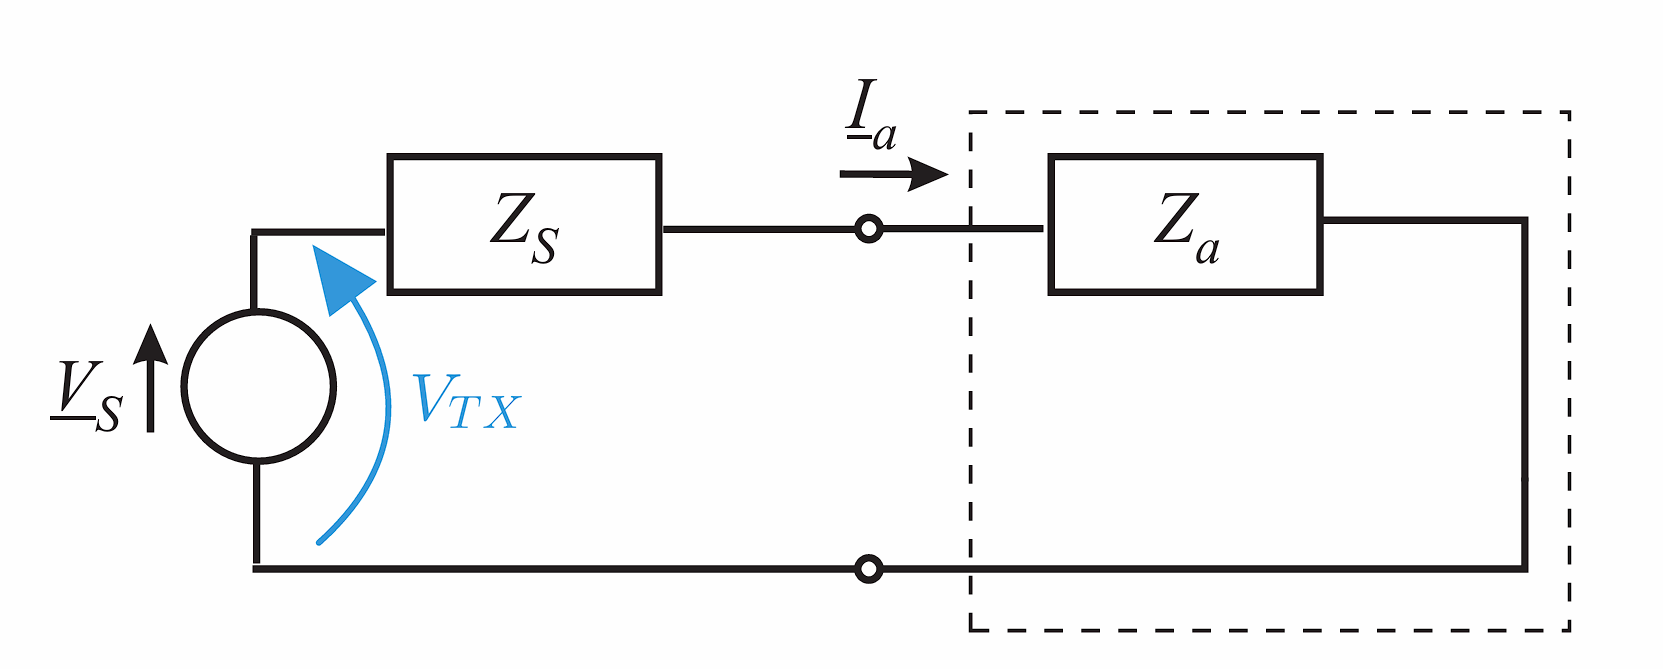
\includegraphics[width=\linewidth]{content/4-images/ant-recep.png}
		\caption{Transmit antenna equivalent circuit, showing the source voltage $V_S$, source impedance $Z_S$, transmit voltage $V_{TX}$, and antenna current $I_a$.}
		\label{fig:tx_circuit}
	\end{subfigure}
	\hfill
	\begin{subfigure}[t]{0.42\textwidth}
		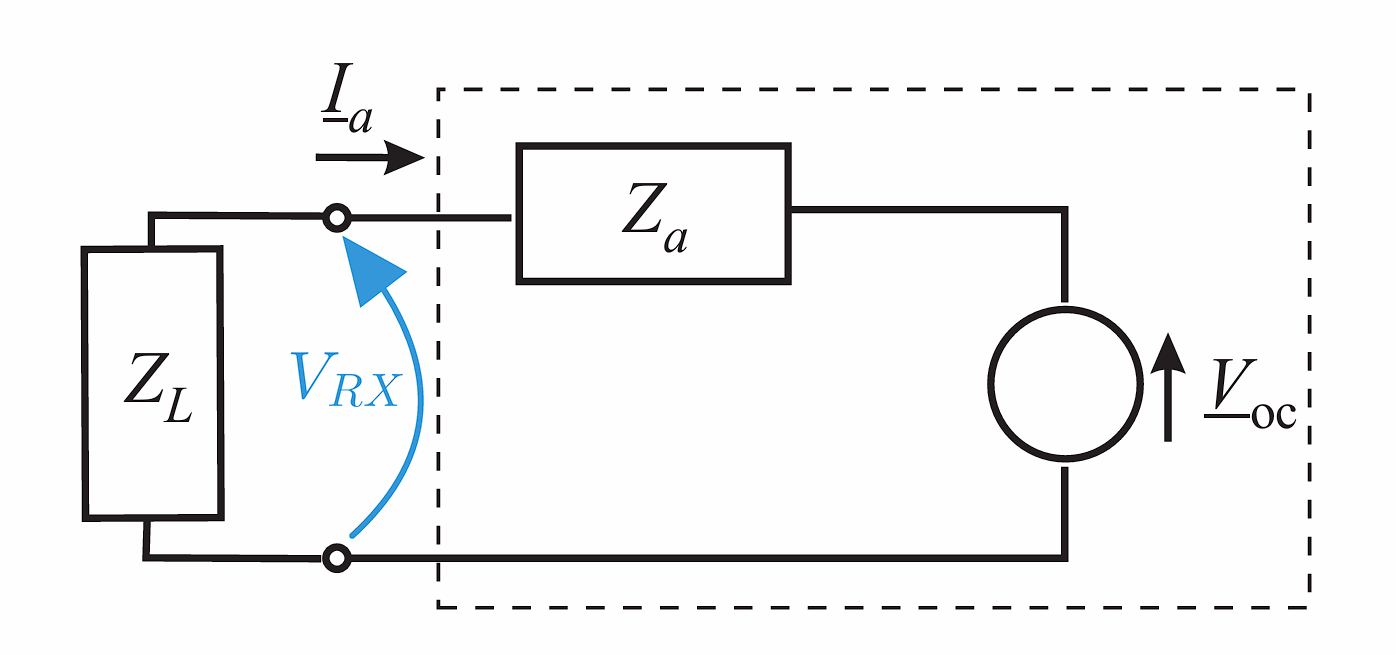
\includegraphics[width=\linewidth]{content/4-images/ant-trans.png}
		\caption{Receive antenna equivalent circuit, showing the induced open-circuit voltage $V_{oc}$, the load impedance $Z_L$, and the received voltage $V_{RX}$.}
		\label{fig:rx_circuit}
	\end{subfigure}
	\caption{Equivalent circuits for the transmit and receive antennas}
	\label{fig:equivalent_circuits}
\end{figure}

The equivalent circuits for the transmitter and receiver are drawn in Figure \ref{fig:equivalent_circuits}. In Figure \ref{fig:tx_circuit}, can be seen the equivalent circuit of the transmitter. The voltage source $V_S$ with its internal impedance $Z_S$ drives the antenna, resulting in a current $I_a$ and a voltage $V_{TX}$ at the antenna's input terminals. At the receiver (Figure \ref{fig:rx_circuit}), the incoming wave induces an open-circuit voltage $V_{oc}$, which in turn produces the received voltage $V_{RX}$ across the load impedance $Z_L$.

For this project, it was considered that the electronics are perfectly matched to the antennas. This implies that for the transmitter, the source impedance is the complex conjugate of the antenna impedance:
\begin{equation}
	Z_S = Z_a^*
\end{equation}
\vspace{0.5em}
and for the receiver, the load impedance is the complex conjugate of the antenna impedance:
\begin{equation}
	Z_L = Z_a^*
\end{equation}
\vspace{0.5em}
This consideration ensures maximum power transfer.

\section{Antenna Effective Height}
\begin{figure}[H]
	\centering
	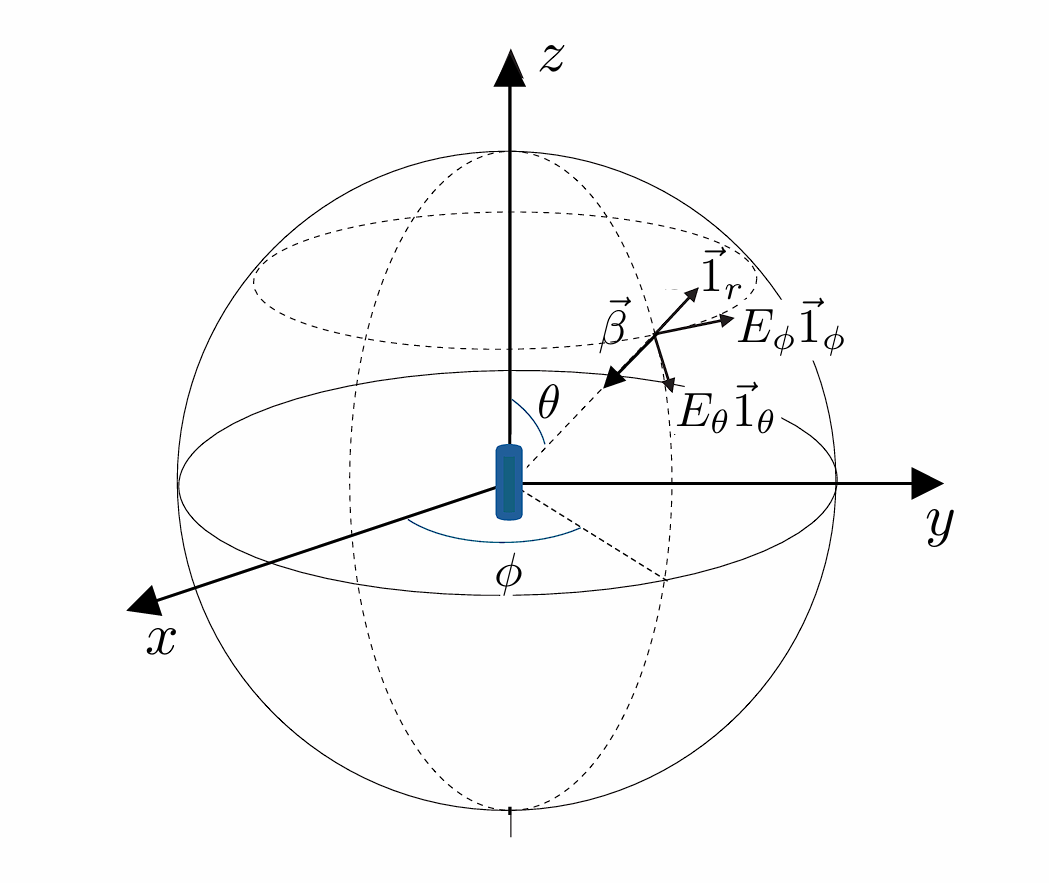
\includegraphics[width=0.5\linewidth]{content/4-images/axes.png}
	\caption{Illustration of the vertical dipole antenna and coordinate axes.}
	\label{fig:axes}
\end{figure}

The effective height $\vec{h}_e$ of an antenna links the circuit domain to the electromagnetic wave domain. It is derived from the current distribution $\vec{J}(\vec{r}\hspace{0.2em}')$ on the antenna when transmitting with an input current $\underline{I}_a$:
\begin{equation}
	\vec{h}_e(\theta, \phi) = \frac{1}{\underline{I}_a} \int_{\mathcal{D}} \vec{J}(\vec{r}\hspace{0.2em}') e^{j\beta(\vec{r}\hspace{0.2em}' \cdot \vec{1}_r)} dV'
	\label{eq:he_general}
\end{equation}
\vspace{0.5em}
where $\mathcal{D}$ is the volume of the antenna, $\vec{1}_r$ is the unit vector in the direction of radiation $(\theta, \phi)$, and $\beta$ is the wavenumber:
\begin{equation}
	\beta = \frac{2\pi}{\lambda}
\end{equation}

For a thin, vertical half-wave dipole antenna of length $L=\frac{\lambda}{2}$ oriented along the z-axis and centered at the origin (Figure \ref{fig:axes}), the current flows only in the z-direction. The current distribution is given by:
\begin{equation}
	\vec{J}(\vec{r}\hspace{0.2em}') = \underline{I}_a \cos(\beta z') \delta(x') \delta(y') \vec{1}_z, \quad \text{for } -\frac{\lambda}{4} \le z' \le \frac{\lambda}{4}
\end{equation}
\vspace{0.5em}
where $\delta(x')$ and $\delta(y')$ are Dirac's deltas.

The volume integral reduces to a line integral along the z-axis. The dot product in the exponent simplifies to:
\begin{equation}
	\vec{r}\hspace{0.2em}' \cdot \vec{1}_r = z' \cos\theta
\end{equation}
\vspace{0.5em}
Substituting this into Equation \ref{eq:he_general} gives:
\begin{equation}
	\vec{h}_e(\theta, \phi) = \left( \int_{-\frac{\lambda}{4}}^{\frac{\lambda}{4}} \cos(\beta z') e^{j\beta z' \cos\theta} dz' \right) \vec{1}_z
	\label{eq:he_integral_form}
\end{equation}
\vspace{0.5em}
The integral in Equation \ref{eq:he_integral_form} is solved using Euler's formula:
\begin{equation}
	\cos(\beta z') = \frac{1}{2}(e^{j\beta z'} + e^{-j\beta z'})
\end{equation}
\begin{align}
	\int_{-\frac{\lambda}{4}}^{\frac{\lambda}{4}} \cos(\beta z') e^{j\beta z' \cos\theta} dz' &= \frac{1}{2} \int_{-\frac{\lambda}{4}}^{\frac{\lambda}{4}} \left( e^{j\beta z'(1+\cos\theta)} + e^{j\beta z'(\cos\theta-1)} \right) dz' \\[\jot]
	&= \frac{1}{2j\beta} \left[ \frac{e^{j\beta z'(1+\cos\theta)}}{1+\cos\theta} + \frac{e^{j\beta z'(\cos\theta-1)}}{\cos\theta-1} \right]_{-\frac{\lambda}{4}}^{\frac{\lambda}{4}}
\end{align}
\vspace{1em}
With $\beta = \frac{2\pi}{\lambda}$, the term $\frac{\beta\lambda}{4}$ simplifies to $\frac{\pi}{2}$. Evaluating at the limits yields:
\vspace{1em}
\begin{align}
	&= \frac{1}{2j\beta} \left[ \frac{e^{j\frac{\pi}{2}(1+\cos\theta)} - e^{-j\frac{\pi}{2}(1+\cos\theta)}}{1+\cos\theta} - \frac{e^{j\frac{\pi}{2}(1-\cos\theta)} - e^{-j\frac{\pi}{2}(1-\cos\theta)}}{1-\cos\theta} \right]
\end{align}

\vspace{1em}
Using the definition of sine: $\sin(x) = \frac{e^{jx}-e^{-jx}}{2j}$

\begin{align}
	&= \frac{1}{\beta} \left[ \frac{\sin\left(\frac{\pi}{2}(1+\cos\theta)\right)}{1+\cos\theta} - \frac{\sin\left(\frac{\pi}{2}(\cos\theta-1)\right)}{1-\cos\theta} \right] \\[\jot]
	&= \frac{1}{\beta} \left[ \frac{\sin(\frac{\pi}{2}+\frac{\pi}{2}\cos\theta)}{1+\cos\theta} + \frac{\sin(\frac{\pi}{2}-\frac{\pi}{2}\cos\theta)}{1-\cos\theta} \right]
\end{align}
\vspace{1em}
Applying the identities $\sin(\frac{\pi}{2}+x) = \cos(x)$ and $\sin(\frac{\pi}{2}-x) = \cos(x)$:
\vspace{1em}
\begin{align}
	&= \frac{1}{\beta} \left[ \frac{\cos(\frac{\pi}{2}\cos\theta)}{1+\cos\theta} + \frac{\cos(\frac{\pi}{2}\cos\theta)}{1-\cos\theta} \right] \\[\jot]
	&= \frac{\cos(\frac{\pi}{2}\cos\theta)}{\beta} \left[ \frac{(1-\cos\theta) + (1+\cos\theta)}{(1+\cos\theta)(1-\cos\theta)} \right] = \frac{2\cos(\frac{\pi}{2}\cos\theta)}{\beta\sin^2\theta}
\end{align}
\vspace{1em}
Substituting $\beta=\frac{2\pi}{\lambda}$, the final result of the integral is:
\begin{equation}
	\frac{\lambda}{\pi} \frac{\cos(\frac{\pi}{2}\cos\theta)}{\sin^2\theta}
\end{equation}
\vspace{0.5em}
The effective height for the vertical half-wave dipole is therefore:
\begin{equation}
	\vec{h}_e(\theta, \phi) = \frac{\lambda}{\pi} \frac{\cos(\frac{\pi}{2}\cos\theta)}{\sin^2\theta} \vec{1}_z
	\label{eq:he_dipole_z}
\end{equation}
\vspace{0.5em}
This vector is oriented along the z-axis. For reception, the induced voltage depends on the component of the effective height that is transverse (perpendicular) to the direction of wave propagation, $\vec{1}_r$. This transverse component is denoted $\vec{h}_{e\perp}$. The Cartesian unit vector $\vec{1}_z$ is expressed in spherical coordinates as:
\begin{equation}
	\vec{1}_z = \cos\theta \vec{1}_r - \sin\theta \vec{1}_\theta
\end{equation}
\vspace{0.5em}
The transverse part, $\vec{h}_{e\perp}$, consists of the components in the $\vec{1}_\theta$ and $\vec{1}_\phi$ directions. Substituting the spherical representation of $\vec{1}_z$ into Equation \ref{eq:he_dipole_z} and retaining only the transverse component gives:
\begin{equation}
	\vec{h}_{e\perp}(\theta, \phi) = -\frac{\lambda}{\pi} \frac{\cos(\frac{\pi}{2}\cos\theta)}{\sin^2\theta} (\sin\theta \vec{1}_\theta) = -\frac{\lambda}{\pi} \frac{\cos(\frac{\pi}{2}\cos\theta)}{\sin\theta} \vec{1}_\theta
	\label{eq:he_perp_general}
\end{equation}
\vspace{0.5em}
This is the general expression for the transverse effective height of a vertical $\frac{\lambda}{2}$ dipole. In the horizontal plane, where $\theta = \frac{\pi}{2}$, the expression simplifies significantly. The transverse effective height in the horizontal plane is therefore:
\begin{equation}
	\boxed{\vec{h}_{e\perp}\left(\theta=\frac{\pi}{2}, \phi\right) = -\frac{\lambda}{\pi} \vec{1}_\theta}
	\label{eq:he_perp_horizontal}
\end{equation}
\vspace{0.5em}
This final expression indicates that in the horizontal plane, the antenna's effective height has a constant magnitude of $\frac{\lambda}{\pi}$, is constant for all $\phi$, and is oriented in the $\vec{1}_\theta$ direction.

\section{Emitted Electric Field in Free-Space}
The electric field radiated by an antenna is given by:
\begin{equation}
	\underline{\vec{E}}(\vec{r}) = -j\omega \underline{I}_a \frac{\mu_0}{4\pi} \frac{e^{-j\beta r}}{r} \vec{h}_{e\perp}(\theta, \phi)
\end{equation}
\vspace{0.5em}
Substituting the transverse effective height for the horizontal plane (Equation \ref{eq:he_perp_horizontal}) into the general expression gives:
\begin{equation}
	\underline{\vec{E}}(r, \pi/2, \phi) = -j\omega \underline{I}_a \frac{\mu_0}{4\pi} \frac{e^{-j\beta r}}{r} \left(-\frac{\lambda}{\pi} \vec{1}_\theta\right) = j \underline{I}_a \frac{\omega \mu_0 \lambda}{4\pi^2} \frac{e^{-j\beta r}}{r} \vec{1}_\theta
\end{equation}
\vspace{0.5em}
Expressing this field in terms of circuit parameters involves the substitutions $\omega = 2\pi f_c$, $\lambda = \frac{c}{f_c}$, $\mu_0 = \frac{Z_0}{c}$, and propagation delay $\tau = \frac{r}{c}$. The exponential term becomes:
\begin{equation}
	e^{-j\beta r} = e^{-j\frac{2\pi}{\lambda}c\tau} = e^{-j2\pi f_c \tau}
\end{equation}
\vspace{0.5em}
The electric field is then:
\begin{equation}
	\underline{\vec{E}} = j \underline{I}_a \frac{(2\pi f_c) (\frac{Z_0}{c}) (\frac{c}{f_c})}{4\pi^2} \frac{e^{-j2\pi f_c \tau}}{c\tau} \vec{1}_\theta = j \underline{I}_a \frac{Z_0}{2\pi c\tau} e^{-j2\pi f_c \tau} \vec{1}_\theta
\end{equation}
\vspace{0.5em}
A half-wave dipole at its resonant frequency has an almost purely real impedance, meaning its reactance is negligible ($X_a \approx 0$), so $Z_a = R_a + jX_a \approx R_a$. Under the perfect matching condition ($Z_S = Z_a^*$), the total impedance in the transmitter circuit is $Z_S + Z_a \approx Z_a^* + Z_a \approx 2R_a$. The antenna current is then related to the transmit voltage by:
\begin{equation}
	\underline{I}_a = \frac{\underline{V}_{TX}}{2R_a}
\end{equation}
\vspace{0.5em}
Substituting this for $\underline{I}_a$:
\begin{equation}
	\boxed{\underline{\vec{E}} = j \frac{Z_0}{4\pi R_a c\tau} \underline{V}_{TX} e^{-j2\pi f_c \tau} \vec{1}_\theta}
	\label{eq:E_field_final}
\end{equation}

\section{Received Voltage in Free-Space}
The open-circuit voltage $\underline{V}_{oc}$ induced at the terminals of a receiving antenna is given by the dot product of its effective height and the incident electric field:
\begin{equation}
	\underline{V}_{oc} = -\vec{h}_{e\perp}^{RX} \cdot \underline{\vec{E}}
\end{equation}
\vspace{0.5em}
The receiving antenna is also a vertical $\frac{\lambda}{2}$ dipole, so its transverse effective height in the horizontal plane is given by Equation \ref{eq:he_perp_horizontal}. The incident electric field is given by Eq. \ref{eq:E_field_final}. The dot product is:
\vspace{1em}
\begin{align}
	\underline{V}_{oc} &= -\left(-\frac{\lambda}{\pi} \vec{1}_\theta\right) \cdot \left(j \frac{Z_0}{4\pi R_a c\tau} \underline{V}_{TX} e^{-j2\pi f_c \tau} \vec{1}_\theta\right) \\[\jot]
	&= j \frac{\lambda Z_0}{4\pi^2 R_a c\tau} \underline{V}_{TX} e^{-j2\pi f_c \tau}
\end{align}
\vspace{1em}
The voltage $\underline{V}_{RX}$ across the receiver load $Z_L$ is found using a voltage divider on the receiver equivalent circuit (Figure \ref{fig:rx_circuit}):
\begin{equation}
	\underline{V}_{RX} = \underline{V}_{oc} \frac{Z_L}{Z_a + Z_L}
\end{equation}
\vspace{0.5em}
With perfect matching ($Z_L = Z_a^*$) and a resonant dipole ($Z_a \approx R_a$), the total impedance in the receiver circuit is $Z_a + Z_L \approx R_a + R_a = 2R_a$. The expression for $\underline{V}_{RX}$ simplifies to:
\begin{equation}
	\underline{V}_{RX} \approx \frac{\underline{V}_{oc}}{2}
\end{equation}
\vspace{0.5em}
Substituting the expression for $\underline{V}_{oc}$ gives the final relationship between the received and transmitted voltages:
\begin{equation}
	\boxed{\underline{V}_{RX} = j \frac{\lambda Z_0}{8\pi^2 R_a c\tau} \underline{V}_{TX} e^{-j2\pi f_c \tau}}
	\label{eq:VRX_vs_VTX}
\end{equation}

\chapter{Line-of-Sight Channel - Narrowband Analysis}
\label{chap:los}

The analysis begins with the simplest communication scenario: a direct Line-of-Sight (LOS) path between the transmitter TX and the receiver RX. A narrowband analysis is conducted, which assumes that the signal's bandwidth is much smaller than the channel's coherence bandwidth. This simplification allows the channel to be characterized by one complex coefficient.

The physical channel can be described by its time-variant impulse response, which for a set of $N$ multipath components is:
\begin{equation}
	h(\tau,t) = \sum_{n=1}^{N} \alpha_n(t) \delta(\tau - \tau_n)
\end{equation}

where $\alpha_n(t)$ and $\tau_n$ are the complex amplitude and propagation delay of the $n$-th path, respectively.

\begin{figure}[H]
	\centering
	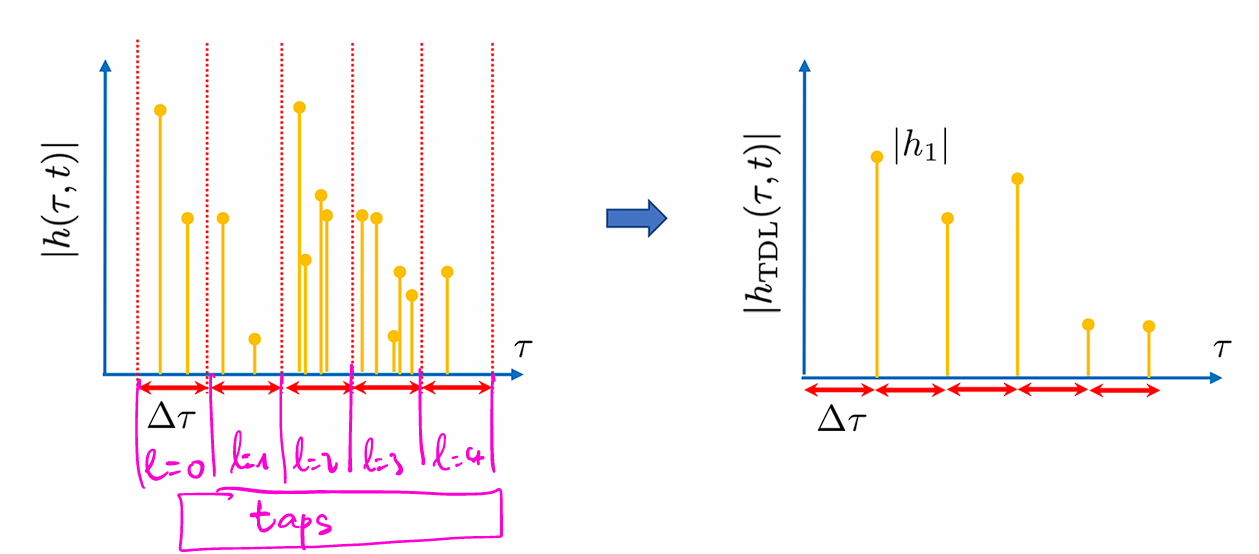
\includegraphics[width=\linewidth]{content/4-images/taps}
	\caption{Physical impulse response and TDL model under the Uncorrelated Scattering assumption}
	\label{fig:taps}
\end{figure}

A practical communication system has a finite bandwidth $B$, which limits its ability to resolve paths arriving at different times. The system's time resolution is $\Delta\tau = 1/B$. 

The received signal is thus defined by:
\begin{equation}
	y(t) = \sum_l x(t-l \Delta \tau) \int_0^{\infty} h(\tau, t) \operatorname{sinc}(B(\tau-l \Delta \tau)) d \tau
\end{equation}

From there, can be defined the complex gain of the $l$-th tap:
\begin{align}
	h_l(t) &= \int_0^{\infty} h(\tau, t) \operatorname{sinc}(B(\tau-l \Delta \tau)) d \tau \\
	&= \int_0^{\infty} (\sum_{n=1}^{N} \alpha_n(t) \delta(\tau - \tau_n)) \cdot \operatorname{sinc}(B(\tau-l \Delta \tau)) d \tau \\
	 &= \sum_{n=1}^N \alpha_n(t) \operatorname{sinc}\left(B\left(\tau_n-l \Delta \tau\right)\right)
\end{align}

\begin{equation}
	\label{eq:h-l}
	\implies \boxed{h_l(t) \approx \sum_{\tau_n \in \operatorname{tap} l} \alpha_n(t)} 
\end{equation}
Equation \ref{eq:h-l} can be written because $\operatorname{sinc(.)}$ maximizes the amplitude of the components of the  $l$-th tap, and the components of other taps are drastically attenuated. The components of the $l$-th tap appear not to be delayed between one another.

The physical limitation of the finite bandwidth of the system leads to the Tapped Delay Line model. The impulse response of the TDL model is a discrete-time representation of the physical channel as shown in Figure \ref{fig:taps}:
\begin{equation}
	h_{TDL}(\tau, t) = \sum_{l=0}^{L} h_l(t) \delta(\tau - l\Delta\tau)
	\label{eq:tdl_model}
\end{equation}


The condition for a narrowband channel is that the signal bandwidth $B$ is much smaller than the channel's coherence bandwidth $\Delta f_c$. The coherence bandwidth is inversely proportional to the channel's delay spread, $\sigma_\tau = max|\tau_i - \tau_j|$. The narrowband condition is thus expressed as:
\begin{equation}
	B \ll \Delta f_c \approx \frac{1}{\sigma_\tau} \implies \Delta\tau \gg \sigma_\tau
\end{equation}

This inequality means the system's time resolution is much larger than the delay spread. From the receiver's perspective, all MPCs arrive at effectively the same time. Consequently, all MPCs fall into the first tap ($l=0$) of the TDL model. The summation in Equation \ref{eq:tdl_model} therefore reduces to one term for $l=0$:
\begin{equation}
	\label{eq:tdl-narrow}
	h_{TDL}(\tau, t) = h_0(t) \delta(\tau)
\end{equation}

where the tap gain $h_0(t)$ is the sum of all individual path gains:
\begin{equation}
	\label{eq:narrow}
	\boxed{h_0(t) = \sum_{n=1}^{N} \alpha_n(t)} \quad N \text{ being the total number of MPCs}
\end{equation}

\section{Antenna Gain}
The gain of an antenna, $G(\theta, \phi)$, quantifies its ability to concentrate radiated power in a specific direction. It is defined by the general formula:
\begin{equation}
	G(\theta,\phi) = \frac{\pi Z_0}{R_a} \frac{|\vec{h}_{e\perp}(\theta,\phi)|^2}{\lambda^2}
	\label{eq:gain_general}
\end{equation}
where $Z_0$ is the impedance of free space, $R_a$ is the antenna's radiation resistance, $\lambda$ is the wavelength, and $\vec{h}_{e\perp}(\theta,\phi)$ is the transverse component of the antenna's effective height.

As derived earlier (Equation \ref{eq:he_perp_horizontal}), the transverse effective height for a vertical half-wave dipole in the horizontal plane ($\theta = \frac{\pi}{2}$) is:
\begin{equation}
	\vec{h}_{e\perp}\left(\frac{\pi}{2},\phi\right) = -\frac{\lambda}{\pi}\vec{1}_{\theta}
\end{equation}

The magnitude squared of this vector is therefore:
\begin{equation}
	\left|\vec{h}_{e\perp}\left(\frac{\pi}{2},\phi\right)\right|^2 = \left|-\frac{\lambda}{\pi}\vec{1}_{\theta}\right|^2 = \frac{\lambda^2}{\pi^2}
\end{equation}

Substituting this result into the general gain formula (Equation \ref{eq:gain_general}) provides the expression for the gain of a lossless half-wave dipole in the horizontal plane:
\begin{equation}
	G = G\left(\frac{\pi}{2}, \phi\right) = \frac{\pi Z_0}{R_a} \frac{1}{\lambda^2} \left(\frac{\lambda^2}{\pi^2}\right) = \frac{\pi Z_0 \lambda^2}{\pi^2 R_a \lambda^2}
\end{equation}
Simplifying this expression yields the final result:
\begin{equation}
	G = \frac{Z_0}{\pi R_a}
	\label{eq:gain_derived}
\end{equation}

\section{Impulse Response $h(\tau)$}
For a single, time-invariant Line-of-Sight path, the channel impulse response is characterized by a single complex amplitude, $\alpha_1$, and a propagation delay, $\tau_1$. The impulse response is thus expressed as:
\begin{equation}
	h(\tau) = \alpha_1 \delta(\tau - \tau_1)
\end{equation}
The central task is to determine the complex amplitude $\alpha_1$. This can be achieved by relating the circuit-level voltages at the transmitter and receiver. The relationship between the transmitted power $P_{TX}$ and the received power $P_{RX}$ is defined by the squared magnitude of the complex amplitude:
\begin{equation}
	P_{RX} = |\alpha_1|^2 P_{TX}
\end{equation}
The transmitted and received powers can be expressed in terms of the terminal voltages $\underline{V}_{TX}$ and $\underline{V}_{RX}$ and the antenna radiation resistance $R_a$, assuming perfectly matched conditions:
\begin{equation}
	P_{TX} = \frac{|\underline{V}_{TX}|^2}{8R_a} \quad \text{and} \quad P_{RX} = \frac{|\underline{V}_{RX}|^2}{2R_a}
\end{equation}
Substituting these power definitions into the power relationship gives:
\begin{equation}
	\frac{|\underline{V}_{RX}|^2}{2R_a} = |\alpha_1|^2 \frac{|\underline{V}_{TX}|^2}{8R_a}
\end{equation}
Solving for $|\alpha_1|^2$ yields:
\begin{equation}
	|\alpha_1|^2 = \frac{8R_a}{2R_a} \frac{|\underline{V}_{RX}|^2}{|\underline{V}_{TX}|^2} = 4 \frac{|\underline{V}_{RX}|^2}{|\underline{V}_{TX}|^2}
\end{equation}
This implies a relationship between the magnitudes: $|\alpha_1| = 2 \frac{|\underline{V}_{RX}|}{|\underline{V}_{TX}|}$. This motivates defining the complex amplitude $\alpha_1$ directly from the complex voltage ratio:
\begin{equation}
	\alpha_1 = 2 \frac{\underline{V}_{RX}}{\underline{V}_{TX}}
	\label{eq:alpha_from_voltages}
\end{equation}
The relationship between the received and transmitted voltages for a free-space LOS path was derived previously (Equation \ref{eq:VRX_vs_VTX}) as:
\begin{equation}
	\underline{V}_{RX} = j \frac{\lambda Z_0}{8\pi^2 R_a c\tau_1} \underline{V}_{TX} e^{-j2\pi f_c \tau_1}
\end{equation}
Substituting this into Equation \ref{eq:alpha_from_voltages} gives the expression for $\alpha_1$:
\begin{equation}
	\alpha_1 = 2 \left( j \frac{\lambda Z_0}{8\pi^2 R_a c\tau_1} e^{-j2\pi f_c \tau_1} \right) = j \frac{\lambda Z_0}{4\pi^2 R_a c\tau_1} e^{-j2\pi f_c \tau_1}
\end{equation}
Replacing the product of the speed of light $c$ and the delay $\tau_1$ with the distance $d_1 = c\tau_1$, the complex amplitude is:
\begin{equation}
	\alpha_1 = j \frac{\lambda Z_0}{4\pi^2 R_a d_1} e^{-j2\pi f_c \tau_1}
	\label{eq:alpha1_derived}
\end{equation}
The channel impulse response for the LOS path is therefore:
\begin{equation}
	h(\tau) = \left( j \frac{\lambda Z_0}{4\pi^2 R_a d_1} e^{-j2\pi f_c \tau_1} \right) \delta(\tau - \tau_1)
	\label{eq:los_impulse_response_derived_detailed}
\end{equation}
where $\tau_1 = d_1/c$.

\section{Transfer Function $H(f)$}
The transfer function $H(f)$ is obtained by taking the Fourier transform of the impulse response $h(\tau)$:
\begin{equation}
	H(f) = \mathcal{FT}\{ h(\tau)\} =  \int_{-\infty}^{\infty} h(\tau) e^{-j2\pi f \tau} d\tau = \int_{-\infty}^{\infty} \left( \alpha_1 \delta(\tau - \tau_1) \right) e^{-j2\pi f \tau} d\tau
\end{equation}
Applying the sifting property of the Dirac delta function, which states that $\int g(x)\delta(x-a)dx = g(a)$, the integral simplifies to:
\begin{equation}
	H(f) = \alpha_1 e^{-j2\pi f \tau_1}
\end{equation}
Substituting the derived expression for $\alpha_1$ from Equation \ref{eq:alpha1_derived}:
\begin{align}
	H(f) &= \left( j \frac{\lambda Z_0}{4\pi^2 R_a d_1} e^{-j2\pi f_c \tau_1} \right) e^{-j2\pi f \tau_1} \\
	\Rightarrow H(f) &= j \frac{\lambda Z_0}{4\pi^2 R_a d_1} e^{-j2\pi (f_c + f) \tau_1}
	\label{eq:los_transfer_function_detailed}
\end{align}
This function shows that the channel introduces a phase shift that is linear with the baseband frequency $f$, which corresponds to the time delay $\tau_1$. The magnitude $|H(f)|$ is constant across all frequencies.

\section{Narrowband Transfer Function $h_{NB}$}
As said mentioned in Equation \ref{eq:tdl-narrow}, the narrowband is defined such that all MPCs fall into a single tap:
\begin{align}
	h_{NB} &= \mathcal{FT}\{ h_{TDL}(t, \tau)\} = \mathcal{FT}\{ h_{0}(t)\delta(\tau)\} \\
	&= \int_{-\infty}^{\infty} h_0(t) e^{-j2\pi f \tau} \delta(\tau) d\tau \\
	&=h_0(t)e^{-j2\pi f \cdot \hspace{0.05em} 0} \\
	\implies h_{NB} &= h_0(t)
\end{align}

As found in Equation \ref{eq:narrow}, for a single LOS path, the narrowband channel transfer function is equal to the complex amplitude $\alpha_1$:
\begin{equation}
	h_{NB} = \sum_{n=1}^{N=1} \alpha_n(t) = \alpha_1
\end{equation}
Using the result from Equation \ref{eq:alpha1_derived}, the narrowband transfer function is:
\begin{equation}
	\boxed{h_{NB} = j \frac{\lambda Z_0}{4\pi^2 R_a d_1} e^{-j2\pi f_c \tau_1}}
	\label{eq:los_narrowband_tf_detailed}
\end{equation}
The LOS channel is thus represented by one complex number, which scales and rotates the transmitted signal.

\section{Received Power $P_{RX}$}
The received power can now be calculated using the derived complex amplitude $\alpha_1$ and its relationship to the power gain, $P_{RX} = |\alpha_1|^2 P_{TX}$. First, the magnitude squared of $\alpha_1$ is computed:
\begin{equation}
	|\alpha_1|^2 = \left| j \frac{\lambda Z_0}{4\pi^2 R_a d_1} e^{-j2\pi f_c \tau_1} \right|^2 = \left( \frac{\lambda Z_0}{4\pi^2 R_a d_1} \right)^2
\end{equation}
Substituting this into the power equation gives the received power as a function of the transmitted power:
\begin{equation}
	P_{RX} = \left( \frac{\lambda Z_0}{4\pi^2 R_a d_1} \right)^2 P_{TX}
\end{equation}
To demonstrate that this result is equivalent to the well-known Friis formula, the terms are rearranged. The expression is factored to isolate terms corresponding to the antenna gains:
\begin{align}
	P_{RX} &= \frac{\lambda^2 Z_0^2}{16\pi^4 R_a^2 d_1^2} P_{TX} \\
	&= \left( \frac{Z_0^2}{\pi^2 R_a^2} \right) \left( \frac{\lambda^2}{16\pi^2 d_1^2} \right) P_{TX} \\
	&= \left( \frac{Z_0}{\pi R_a} \right) \left( \frac{Z_0}{\pi R_a} \right) \left( \frac{\lambda}{4\pi d_1} \right)^2 P_{TX}
\end{align}
Using the expression for the gain of a lossless half-wave dipole in the horizontal plane as derived in Equation \ref{eq:gain_derived}, $G = Z_0/(\pi R_a)$, and assuming identical transmit and receive antennas ($G_{TX} = G_{RX} = G$):
\begin{equation}
	P_{RX} = G_{TX} G_{RX} \left( \frac{\lambda}{4\pi d_1} \right)^2 P_{TX} \label{eq:los_power_final_detailed}
\end{equation}
This result is identical to the Friis transmission formula. This validates the entire derivation, confirming that the complex amplitude $\alpha_1$ derived from the voltage ratio correctly predicts the power relationship under free-space LOS conditions.

\section{Interpretation of Results}
The derivations confirm the principles of a simple LOS communication link.
\begin{itemize}
	\item \textbf{Frequency-Flat Channel:} The single propagation path results in a transfer function $|H(f)|$ that is constant with frequency. This means the channel does not distort the signal's spectrum, a condition known as flat fading. This is a direct consequence of having no time dispersion (zero delay spread).
	\item \textbf{Validation of Friis' Formula:} The derivation, starting from the circuit-level voltage relationship to find the complex amplitude $\alpha_1$, and then using it to find the received power, shows a result identical to the Friis' formula. This demonstrates a consistency between the low-level physical model (fields and circuits) and the high-level system model (power and gains).
\end{itemize}

\chapter{Full Channel, Narrowband Analysis}
\label{chap:full_narrow}

The analysis now expands from the LOS model to a more comprehensive full-channel model. This section considers the impact of multiray components generated by reflections off the buildings lining. The analysis remains within the narrowband regime, where the channel's response can be characterized by a single complex coefficient, but this coefficient now incorporates the vector sum of all significant propagation rays, not just the direct one.


In a realistic urban environment, the signal transmitted from TX to RX does not travel along a single ray. Instead, it propagates along multiple rays due to reflections from surrounding objects, in this case, the building facades. Each of these rays is an MPC. The total received signal is the vector sum of all these MPCs. The narrowband channel transfer function, previously represented by a single complex gain $\alpha_1$ for the LOS ray, is now the sum of the complex gains of all MPCs:
\begin{equation}
	h_{NB} = \sum_{n=1}^{N} \alpha_n
\end{equation}
where $N$ is the total number of MPCs, including the LOS ray and all reflected rays. Each complex gain $\alpha_n$ is a function of the ray's length, the reflection coefficients of the surfaces it interacts with, and the propagation delay.

The primary tool for identifying these rays and calculating their geometry is the \textbf{image method}. For each reflecting surface, an image of the transmitter is created. A straight line from this image to the receiver identifies the ray of the reflected wave, as shown in Figure \ref{fig:image_method_single}. This method can be extended recursively to find rays with multiple reflections.

\begin{figure}[h!]
	\centering
	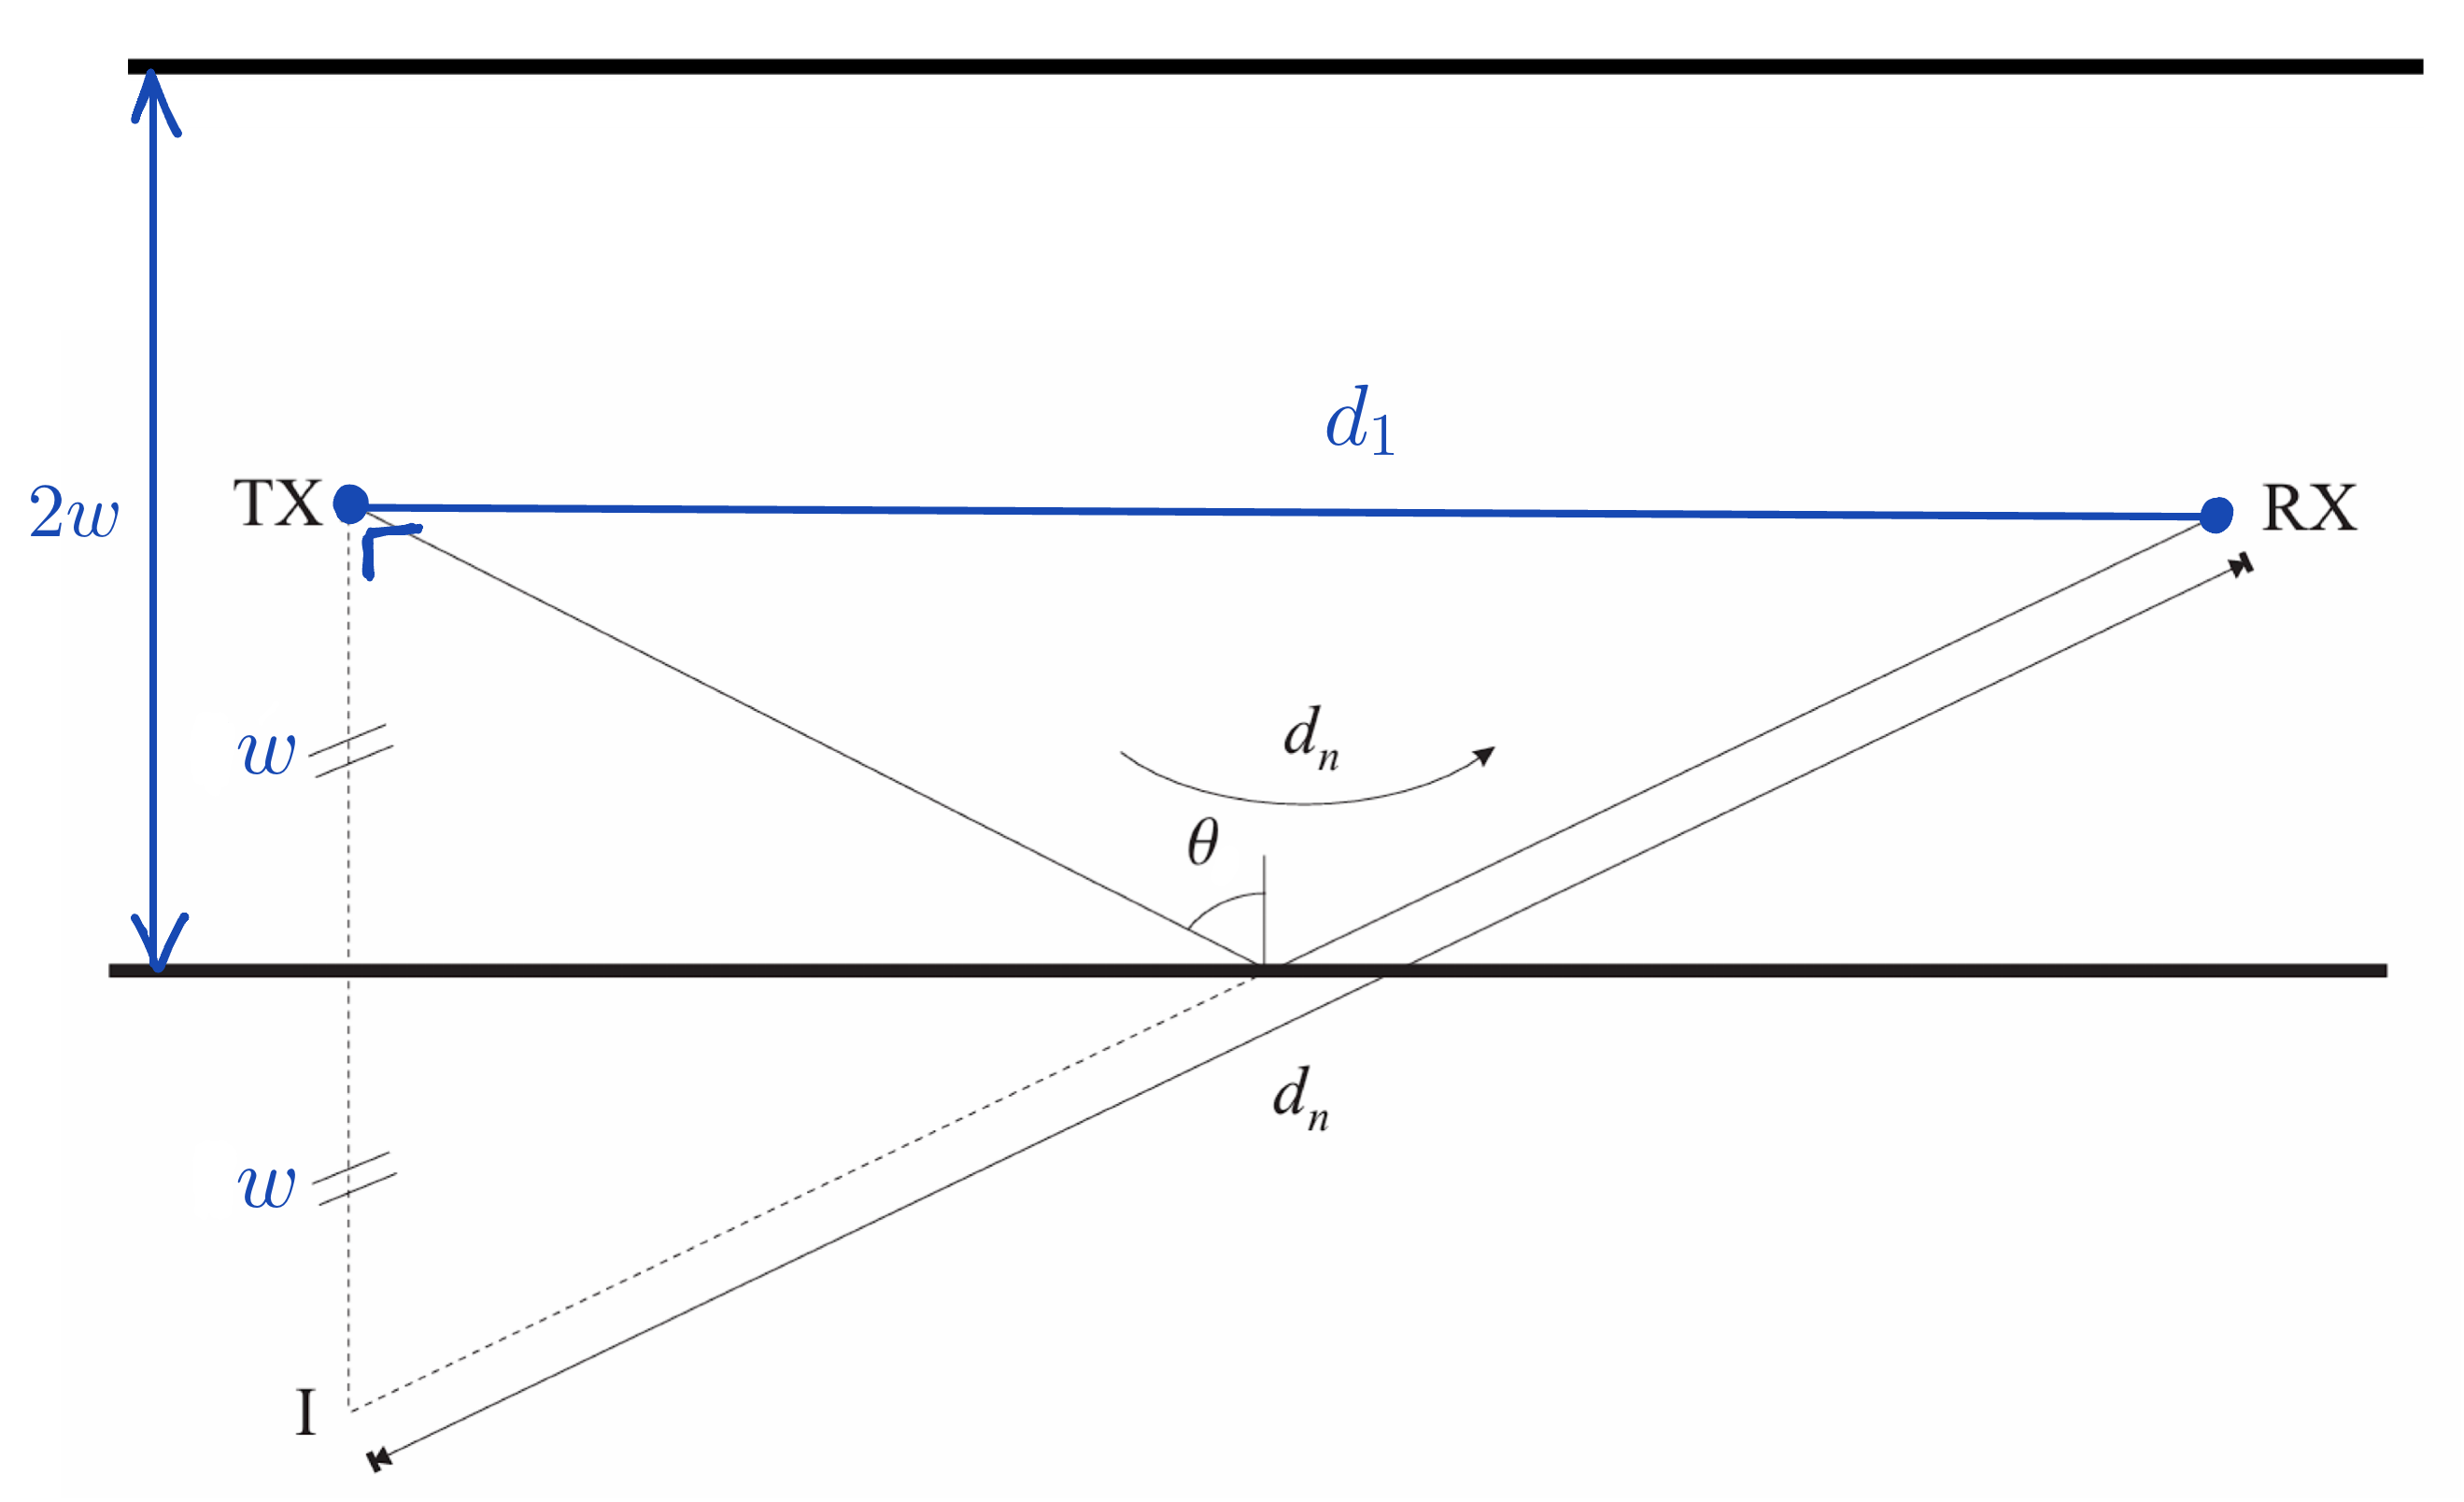
\includegraphics[width=0.7\linewidth]{content/4-images/image-method.png}
	\caption{The image method for a single reflection. The ray of the reflected ray from TX to RX is found by drawing a straight line from the image transmitter I to RX.}
	\label{fig:image_method_single}
\end{figure}


\section{Multiray Component Geometry}
To find the paths of all significant rays, we use the image method. The scenario is a urban street of width $2w = 20$ m. The transmitter TX and receiver RX are placed symmetrically in the center of the street, separated by a distance $d$. The building walls are represented by two parallel lines at $y = w$ and $y = -w$.

\subsubsection{LOS ray}
The LOS ray is the direct, unobstructed path between the transmitter and receiver. It is considered as the first path component, meaning $n=1$.
\begin{itemize}
	\item \textbf{Path Length: $d_1 = d$} The
	\item \textbf{Propagation Delay:}
	\begin{equation}
		\tau_{1} = \frac{d}{c}
	\end{equation}
\end{itemize}

\subsubsection{Single Reflection rays}
There are two distinct paths involving one reflection, one from the top wall and one from the bottom wall. Using the image method, we create a virtual source $I_1$ by reflecting the TX across the wall. The path length is the straight-line distance from $I_1$ to the RX.
\begin{itemize}
	\item \textbf{Path Length:} The geometry forms a right triangle with legs and $d$ and $2w$ (the vertical distance between the image and the RX).
	\begin{equation}
		d_{n} = \sqrt{d^2 + (2w)^2}
	\end{equation}
	\item \textbf{Propagation Delay:}
	\begin{equation}
		\tau_{n} = \frac{\sqrt{d^2 + (2w)^2}}{c}
	\end{equation}
	\item \textbf{Angle of Incidence:} The angle of incidence with the wall is given by:
	\begin{equation}
		\sin(\theta_{n}) = \frac{d}{d_{n}}
	\end{equation}
\end{itemize}

\subsubsection{Double Reflection rays}
There are two paths involving two reflections (e.g. Wall 1 $\rightarrow$ Wall 2 $\rightarrow$ RX). To find the path length, we create a second-order image $I_2$, by reflecting the first-order image $I_1$ across the opposite wall.
\begin{itemize}
	\item \textbf{Path Length:} The vertical separation between the second-order image $I_2$ and the RX is now $4w$.
	\begin{equation}
		d_{n} = \sqrt{d^2 + (4w)^2}
	\end{equation}
	\item \textbf{Propagation Delay:}
	\begin{equation}
		\tau_{n} = \frac{\sqrt{d^2 + (4w)^2}}{c}
	\end{equation}
	 \item \textbf{Angle of Incidence:} The angle of incidence is the same for both reflections and is given by:
	\begin{equation}
		\cos(\theta_{n}) = \frac{d}{d_{n}} = \frac{d}{\sqrt{d^2 + (4w)^2}}
	\end{equation}
\end{itemize}


\subsubsection{K-th Order Reflection Rays (Recursive Approach)}
While closed-form expressions can be derived for this simple geometry, a more robust and general method is to define the process recursively, as implemented in the simulation. To find all paths with up to $K$ reflections, the algorithm extends the image method by systematically generating and validating potential ray paths.

This process is implemented using the recursive function \texttt{findReflectedRaysRecursive}, which builds a tree of image sources as illustrated in Figure \ref{fig:image_tree}. The function starts with the real transmitter (the 0-order source) and the desired number of reflections. In each recursive step, it mirrors the current source across every wall in the environment using \texttt{findSymmetricAcrossLine}, creating a new set of higher-order image sources. It then calls itself for each new image, with the remaining number of reflections decremented. To avoid physically redundant paths, a source is never immediately reflected back across the same wall it was just generated from.

\begin{figure}[h!]
	\centering
	%====================================================================================
	% TIKZ PREAMBLE REQUIREMENTS
	% To compile this figure, ensure you have the following lines in your main .tex file's preamble:
	% \usepackage{tikz}
	% \usetikzlibrary{arrows.meta, positioning}
	% The 'positioning' library is used for the "below left/right=of" syntax.
	%====================================================================================
	\begin{tikzpicture}[
		% Set distances for manual placement
		node distance=1.5cm and 2.5cm,
		% Common style for all nodes in the diagram
		every node/.style={
			shape=rectangle,
			rounded corners,
			draw,
			align=center,
			top color=white,
			bottom color=blue!20
		},
		% Style for the connecting arrows
		arrow/.style={draw, -{Latex[length=2mm]}}
		]
		% Place nodes manually using the 'positioning' library features
		\node (root) {TX (Order 0)};
		\node (c1) [below left=of root] {$I_{W1}$ (Order 1)};
		\node (c2) [below right=of root] {$I_{W2}$ (Order 1)};
		\node (c11) [below=1.5cm of c1] {$I_{W1,W2}$ (Order 2)};
		\node (c21) [below=1.5cm of c2] {$I_{W2,W1}$ (Order 2)};
		\node (c111) [below=of c11] {$\dots$};
		\node (c211) [below=of c21] {$\dots$};
		
		% Draw the arrows and place the styled labels on them
		% The 'node' command here creates a label that inherits the 'every node' style
		\path[arrow] (root.south) -- (c1.north)
		node[midway, sloped, font=\ttfamily] {mirror(TX, W1)};
		\path[arrow] (root.south) -- (c2.north)
		node[midway, sloped, font=\ttfamily] {mirror(TX, W2)};
		
		% Draw the rest of the arrows
		\path[arrow] (c1) -- (c11);
		\path[arrow] (c2) -- (c21);
		\path[arrow] (c11) -- (c111);
		\path[arrow] (c21) -- (c211);
	\end{tikzpicture}
	\caption{Conceptual tree of image sources generated by \texttt{findReflectedRaysRecursive}. Each level corresponds to an order of reflection.}
	\label{fig:image_tree}
\end{figure}

The recursion stops when the desired reflection order is reached. At this point, the sequence of image sources defines a potential ray path. However, this path is only geometrically hypothetical. It must be validated by the \texttt{validateRayPath} function, which traces the path backward from RX to TX. The logic of this validation is detailed in the flowchart in Figure \ref{fig:validation_flowchart}.

\begin{figure}[h!]
	\centering
	%====================================================================================
	% TIKZ PREAMBLE REQUIREMENTS
	% To compile this figure, ensure you have the following lines in your main .tex file's preamble:
	% \usepackage{tikz}
	% \usetikzlibrary{arrows.meta, positioning, shapes.geometric}
	% The 'shapes.geometric' library is essential for the diamond shape.
	%====================================================================================
	\begin{tikzpicture}[
		node distance=1.3cm and 1cm,
		block/.style={rectangle, draw, fill=blue!20, text width=10em, text centered, rounded corners, minimum height=3em},
		line/.style={draw, -{Latex[length=2mm]}},
		decision/.style={diamond, draw, fill=green!20, text width=5.5em, text centered, aspect=1.5, inner sep=0pt}
		]
		% Nodes
		\node [block] (start) {Start with RX,\\ images: ($I_M \dots I_1$); walls: ($W_M \dots W_1$). Let $m=M$.};
		\node [block, below=of start] (intersect) {Cast ray from current point to $I_M$. Find intersection $R_m$ on wall $W_m$.};
		\node [decision, below=of intersect] (dec1) {$R_m$ on wall segment?};
		\node [block, below=of dec1] (obstruct) {Check segment from $R_m$ to previous point for obstructions.};
		\node [decision, below=of obstruct] (dec2) {Obstructed?};
		\node [decision, below=of dec2] (dec3) {$m=1$? (Last segment)};
		\node [block, left=of dec3, xshift=-1cm] (loop) {Decrement $m$. Set $R_m$ as new current point.};
		\node [block, right=of dec1, xshift=1cm, fill=red!30] (invalid1) {Path Invalid};
		\node [block, right=of dec2, xshift=1cm, fill=red!30] (invalid2) {Path Invalid};
		\node [block, below=of dec3, fill=green!30] (valid) {Path Valid!};
		
		% Paths
		\path [line] (start) -- (intersect);
		\path [line] (intersect) -- (dec1);
		\path [line] (dec1) -- node[anchor=east] {Yes} (obstruct);
		\path [line] (dec1) -- node[anchor=south] {No} (invalid1);
		\path [line] (obstruct) -- (dec2);
		\path [line] (dec2) -- node[anchor=south] {Yes} (invalid2);
		\path [line] (dec2) -- node[anchor=east] {No} (dec3);
		\path [line] (dec3) -- node[anchor=east] {Yes} (valid);
		\path [line] (dec3) -- node[anchor=north] {No} (loop);
		\path [line] (loop) |- (intersect);
		
	\end{tikzpicture}
	\caption{Flowchart of the backward path validation process in \texttt{validateRayPath}.}
	\label{fig:validation_flowchart}
\end{figure}

The validation process follows the sequence:
\begin{enumerate}
	\item Starting from the RX, a line is cast to the final image source ($I_M$). Its intersection with the corresponding wall segment ($W_M$) is found using \texttt{findSegmentIntersection}. If an intersection point does not exist on the finite wall segment, the path is invalid.
	\item If the reflection point is valid, the path segment from it to the RX is checked for obstructions by any other wall. If it is obstructed, the path is invalid.
	\item The process is then repeated, tracing backward from the newly found reflection point to the next image in the sequence ($I_{K-1}$) to find the next reflection point on its respective wall ($W_{K-1}$).
	\item This continues until the entire path has been traced back to the original transmitter. A path is only considered valid if every segment is unobstructed and every reflection point lies on its physical wall.
\end{enumerate}

Once $n$-th ray path is validated, the function \texttt{calculatePhysicalProperties} computes its total path length $d_n$, by summing the lengths of its segments. It also calculates the angle of incidence for each reflection to find the product of the Fresnel reflection coefficients.

For the specific symmetric  geometry of the setup, this recursive algorithm correctly identifies the paths whose lengths are given by the simplified formula:
\begin{equation}
	d_{n} = \sqrt{d^2 + (2Mw)^2}
\end{equation}
The corresponding propagation delay is:
\begin{equation}
	\tau_{n} = \frac{\sqrt{d^2 + (2Mw)^2}}{c}
\end{equation}
An the Angle of incidence is defined by:
\begin{equation}
	\cos(\theta_{n}) = \frac{d}{d_{n}} = \frac{d}{\sqrt{d^2 + (2Mw)^2}}
\end{equation}

For a simulation considering up to $M=10$ reflections, this process identifies the LOS ray plus two rays for each reflection order, resulting in a total of $N=1+2\times10=21$ valid MPCs.

\begin{figure}
	\centering
	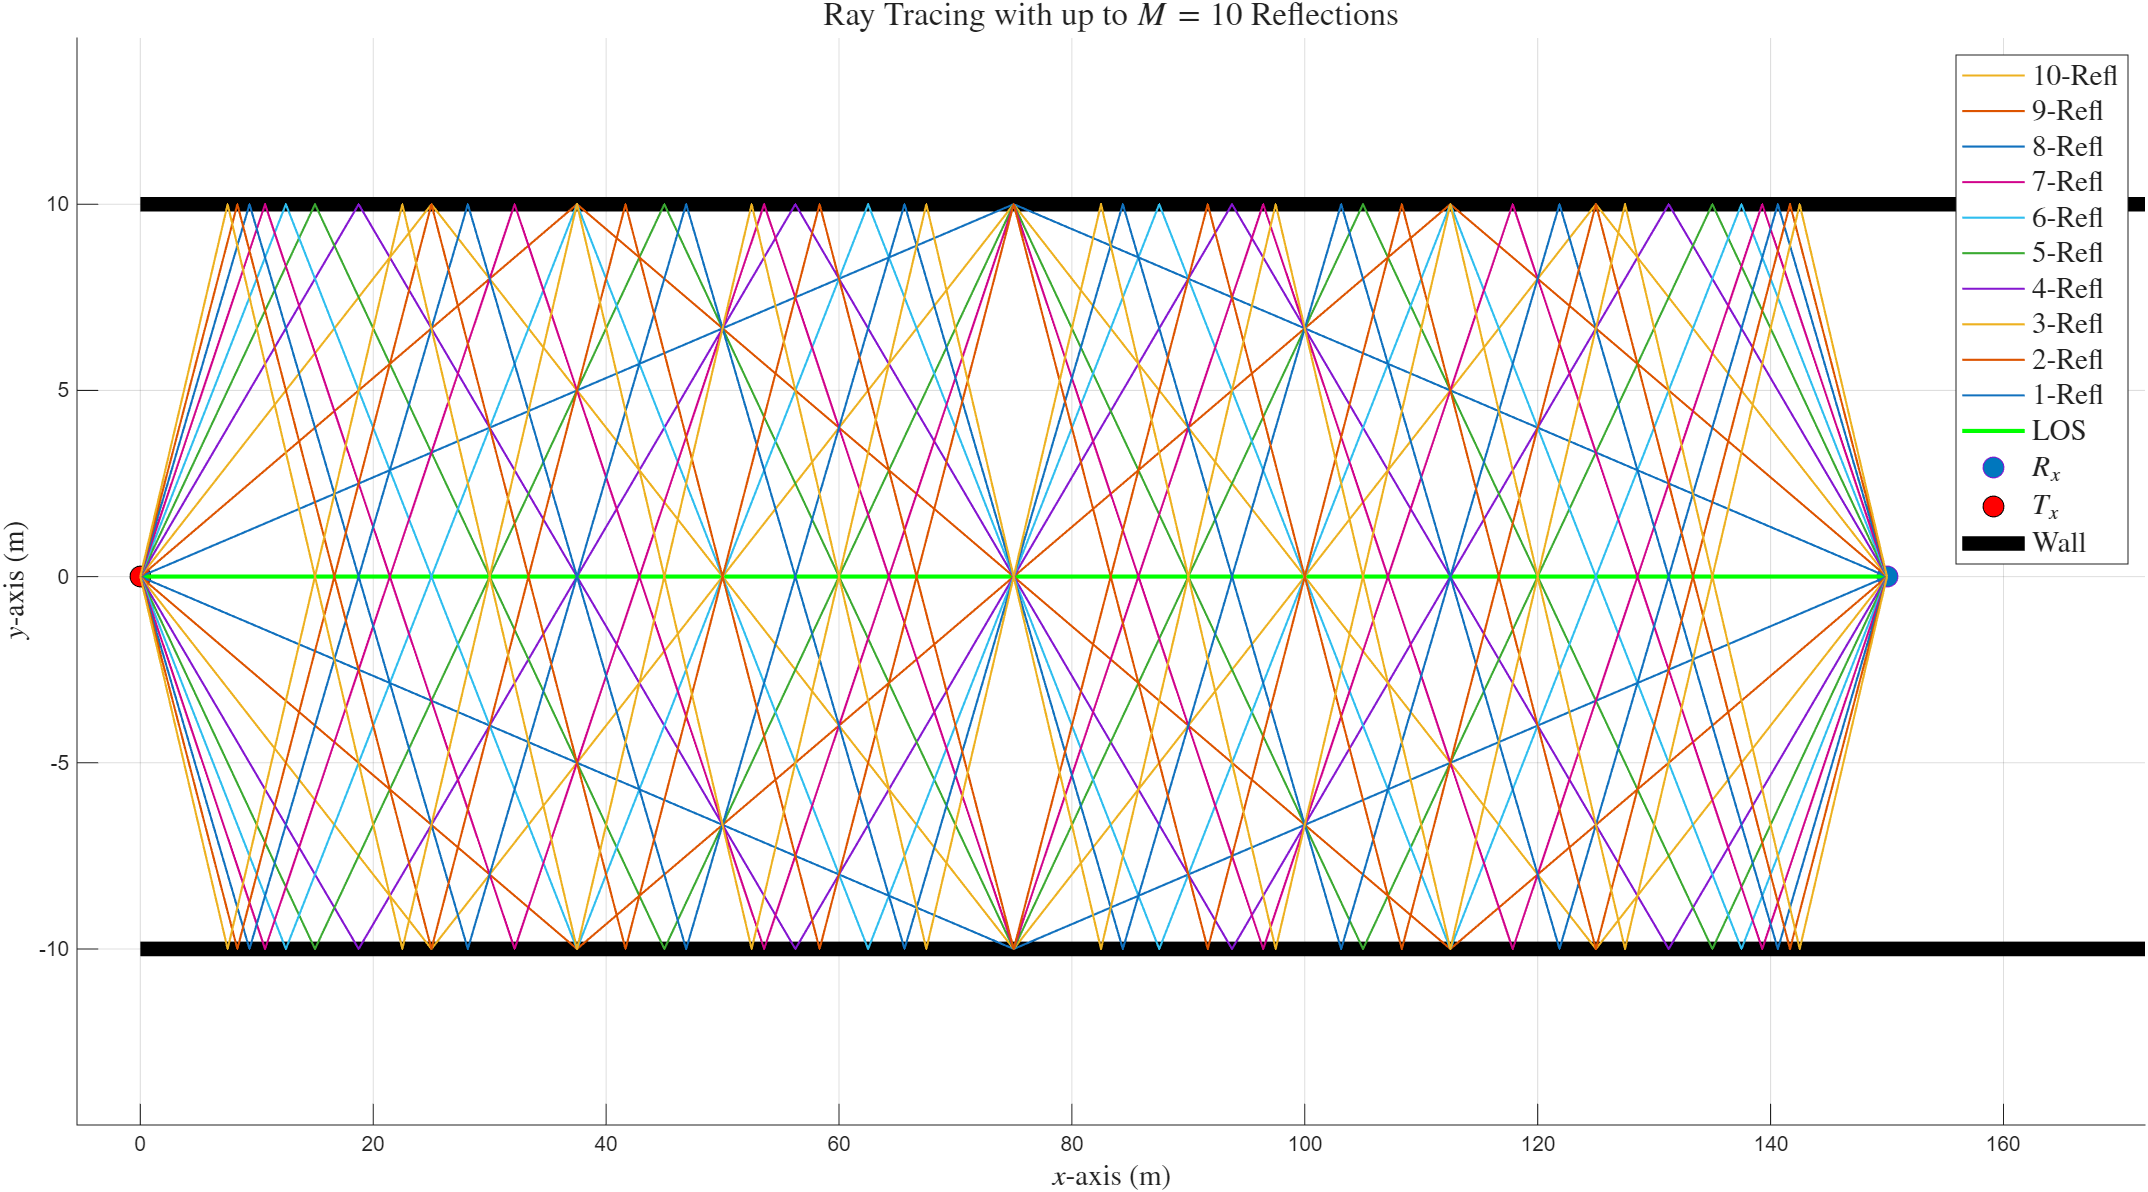
\includegraphics[width=\linewidth]{content/4-images/ray-tracing-10-reflections.png}
	\caption{Simulation of the image method ray-tracing for 10 reflections, showing the 21 valid MPCs found.}
	\label{fig:raytracing-3reflex}
\end{figure}



\section{Total Received Voltage}
The complex amplitude $\alpha_n$ for each ray $n$ must account for the path loss and any phase changes from reflections. The general form for the complex amplitude of a ray of length $d_n$ with $M$ reflections is:
\begin{equation}
	\alpha_n = \left( j \frac{\lambda Z_0}{4\pi^2 R_a d_n} e^{-j2\pi f_c \tau_n} \right) \times \prod_{m=1}^{M}(\Gamma_{\perp, m}(\theta_{n}))
\end{equation}
where $\Gamma_{\perp}$ is the reflection coefficient for perpendicular polarization for the $n$-th MPC experiencing $M$ reflections:
\begin{equation}
	\Gamma_{\perp, m}(\theta_n) = \frac{\cos\theta_n - \sqrt{\epsilon_{r, m} - \sin^2\theta_n}}{\cos\theta_n + \sqrt{\epsilon_{r, m} - \sin^2\theta_m}}
\end{equation}
with $\epsilon_{r,m} = 4$ for the buildings. The angle of incidence $\theta_n$ is specific to each reflection order.

The narrowband transfer function found in Equation \eqref{eq:narrow} is given by :
\begin{equation}
	h_{NB} = \sum_{n=1}^{N=7} \alpha_n = \alpha_{LOS} + \sum_{n=2}^{N=7} \alpha_n
\end{equation}

The total received voltage $\underline{V}_{RX}$ is then:
\begin{equation}
	\underline{V}_{RX} = \frac{h_{NB}}{2} \underline{V}_{TX}
\end{equation}

\section{Received Power and Comparison with Friis Formula}

The received power is:
\begin{equation}
	P_{RX} = |h_{NB}|^2 P_{TX} = \left| \alpha_{LOS} + \sum_{n=2}^{N=7} \alpha_n \right|^2 P_{TX}
\end{equation}
This expression highlights the difference from the LOS only represented by the Friis formula:
\begin{equation}
	P_{RX, \text{Friis}} = P_{TX} G_{TX} G_{RX} \left( \frac{\lambda}{4\pi d} \right)^2 = |\alpha_{LOS}|^2 P_{TX}
\end{equation}
The Friis formula represents the power of only the first term ($n=1$) in the sum. In the full channel model, the total power depends on the vector sum of all 7 MPCs. Because the rays have different lengths $d_n$ and undergo different phase shifts ($e^{-j2\pi f_c \tau_n}$ and from reflections), the complex amplitudes $\alpha_n$ add up coherently.

\begin{figure}[H]
	\centering
	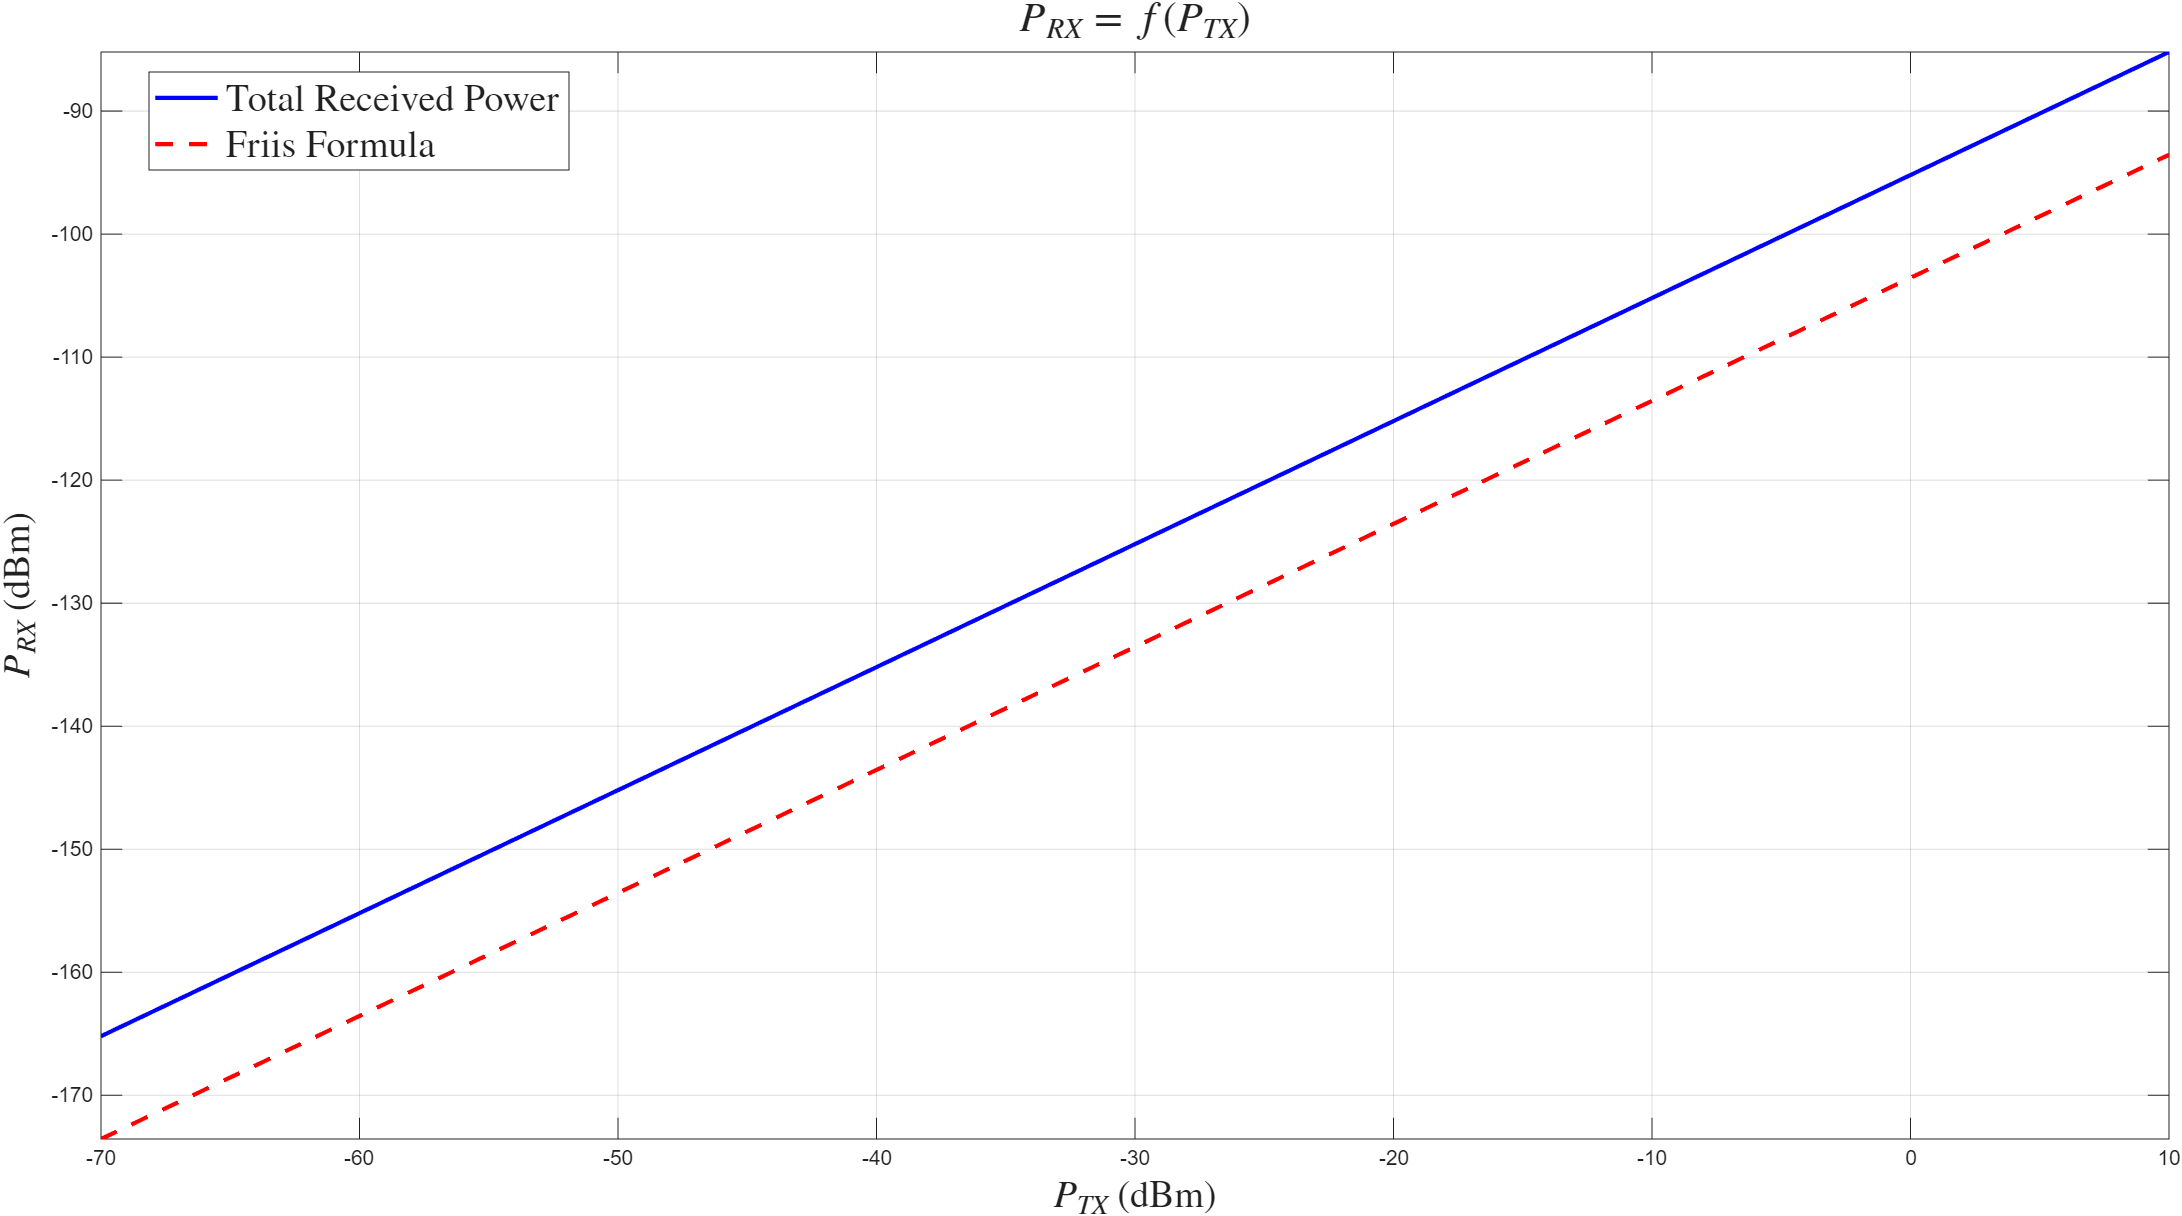
\includegraphics[width=1\linewidth]{content/4-images/PRX-vs-PTX}
	\caption{Received Power as a function of the Transmitted Power for a fixed channel ($d$ is constant and equal to $1km$). The number of reflections is $M=10$}
	\label{fig:prx-vs-ptx}
\end{figure}


This coherent summation results in fast fading for small distances and slow fading for very high distances between TX and RX. \\
Unlike the monotonic decrease of power with all distances predicted by the Friis formula, the full-channel received power will exhibit significant fluctuations as the distance $d$ changes at smaller distances. As seen in Figure \ref{fig:pRX_vs_friis}, for very high values of d, the models gets closer to the Friis formula, because the reflected rays will be drastically attenuated, compared to the LOS ray
\begin{itemize}
	\item \textbf{Constructive Interference:} At locations where the MPCs arrive largely in-phase, their amplitudes add up, resulting in a received power that can be significantly higher than the Friis prediction.
	\item \textbf{Destructive Interference:} At locations where some MPCs arrive out-of-phase, their amplitudes cancel each other out, leading to drops far below the Friis prediction.
\end{itemize}

\begin{figure}[h!]
	\centering
	% You should generate this plot using simulation tools (e.g., MATLAB, Python)
	% based on the derived equations for the 7 MPCs.
	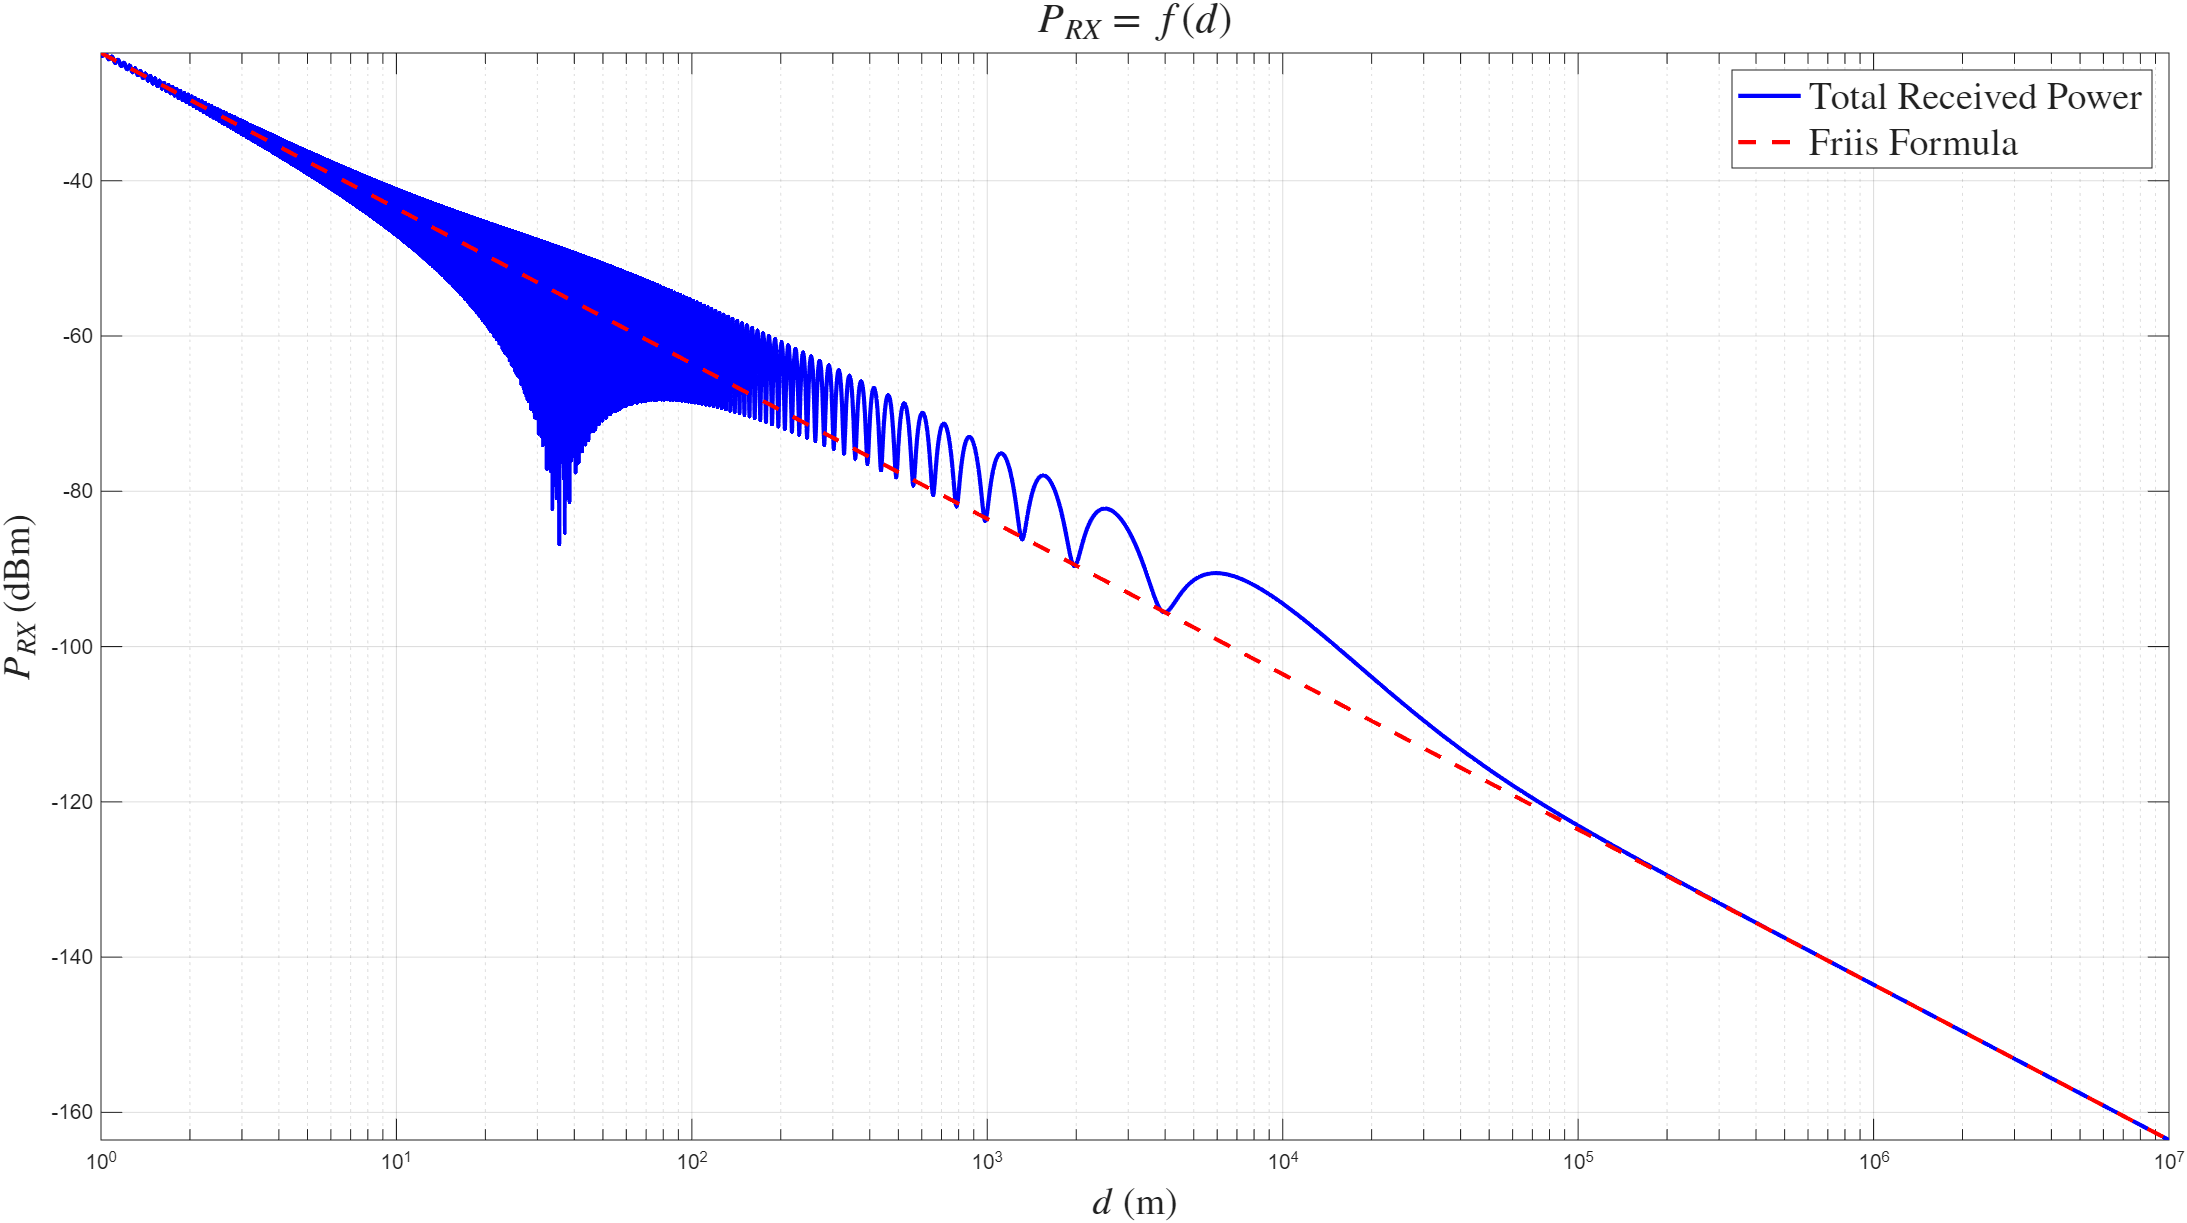
\includegraphics[width=\linewidth]{content/4-images/PRX-vs-Friis.png} % Placeholder ray
	\caption{Received power as a function of the separation distance between TX and RX in the Multipath Narrow band scenario for $M=1$ Reflection}
	\label{fig:pRX_vs_friis}
\end{figure}

\section{Rician factor}
The Rician factor $K$ is a parameter that quantifies the severity of fading in a channel. 
\begin{equation}
	K = \frac{|\alpha_{LOS}|^2}{\sum_{n=2}^{7} |\alpha_n|^2} = \frac{P_{LOS}}{P_{NLOS}}
\end{equation}
To evaluate this, we need to express $|\alpha_n|^2$ in terms of physical parameters. From the LOS analysis made earlier, we found that the received power for the direct ray is identical to the Friis formula:
\begin{equation}
	P_{LOS} = |\alpha_{LOS}|^2 P_{TX} = G_{TX} G_{RX} \left( \frac{\lambda}{4\pi d} \right)^2 P_{TX}
\end{equation}
This gives us the power gain for the LOS component ($d_1 = d$, $|\Gamma_1|^2=1$):
\begin{equation}
	|\alpha_{LOS}|^2 = G_{TX} G_{RX} \left( \frac{\lambda}{4\pi d} \right)^2
\end{equation}
For the $n$-th MPC that is not the LOS ray, and experiences reflections, the power is reduced by the cumulative reflection coefficient $\Gamma_n = \prod_{m=1}^{M}(\Gamma_{\perp, m}(\theta_{n}))$. The power gain for a reflected ray of total travel distance $d_n$ is therefore:
\begin{equation}
	|\alpha_n|^2 = G_{TX} G_{RX} \left( \frac{\lambda}{4\pi d_n} \right)^2 |\Gamma_n|^2
\end{equation}

Substituting these expressions for power gain into the K-factor equation:
\begin{equation}
	K = \frac{G_{TX} G_{RX} \left( \frac{\lambda}{4\pi d} \right)^2}{\sum_{n=2}^{7} G_{TX} G_{RX} \left( \frac{\lambda}{4\pi d_n} \right)^2 |\Gamma_n|^2}
\end{equation}
The common terms, including antenna gains and wavelength, cancel out, leaving a purely geometric relationship:
\begin{equation}
	K = \frac{\frac{1}{d^2}}{\sum_{n=2}^{7} \frac{|\Gamma_n|^2}{d_n^2}} \implies \boxed{K =\frac{1}{d^2 \sum_{n=2}^{7} \frac{|\Gamma_n|^2}{d_n^2}}}
\end{equation}
A high K-factor indicates that the channel is dominated by the LOS ray, and fading will be less severe leading to the Rician distribution. A low K-factor indicates that the NLOS rays are stronger relative to the LOS ray, leading to deep fades characteristic of Rayleigh distribution.

\begin{figure}
	\centering
	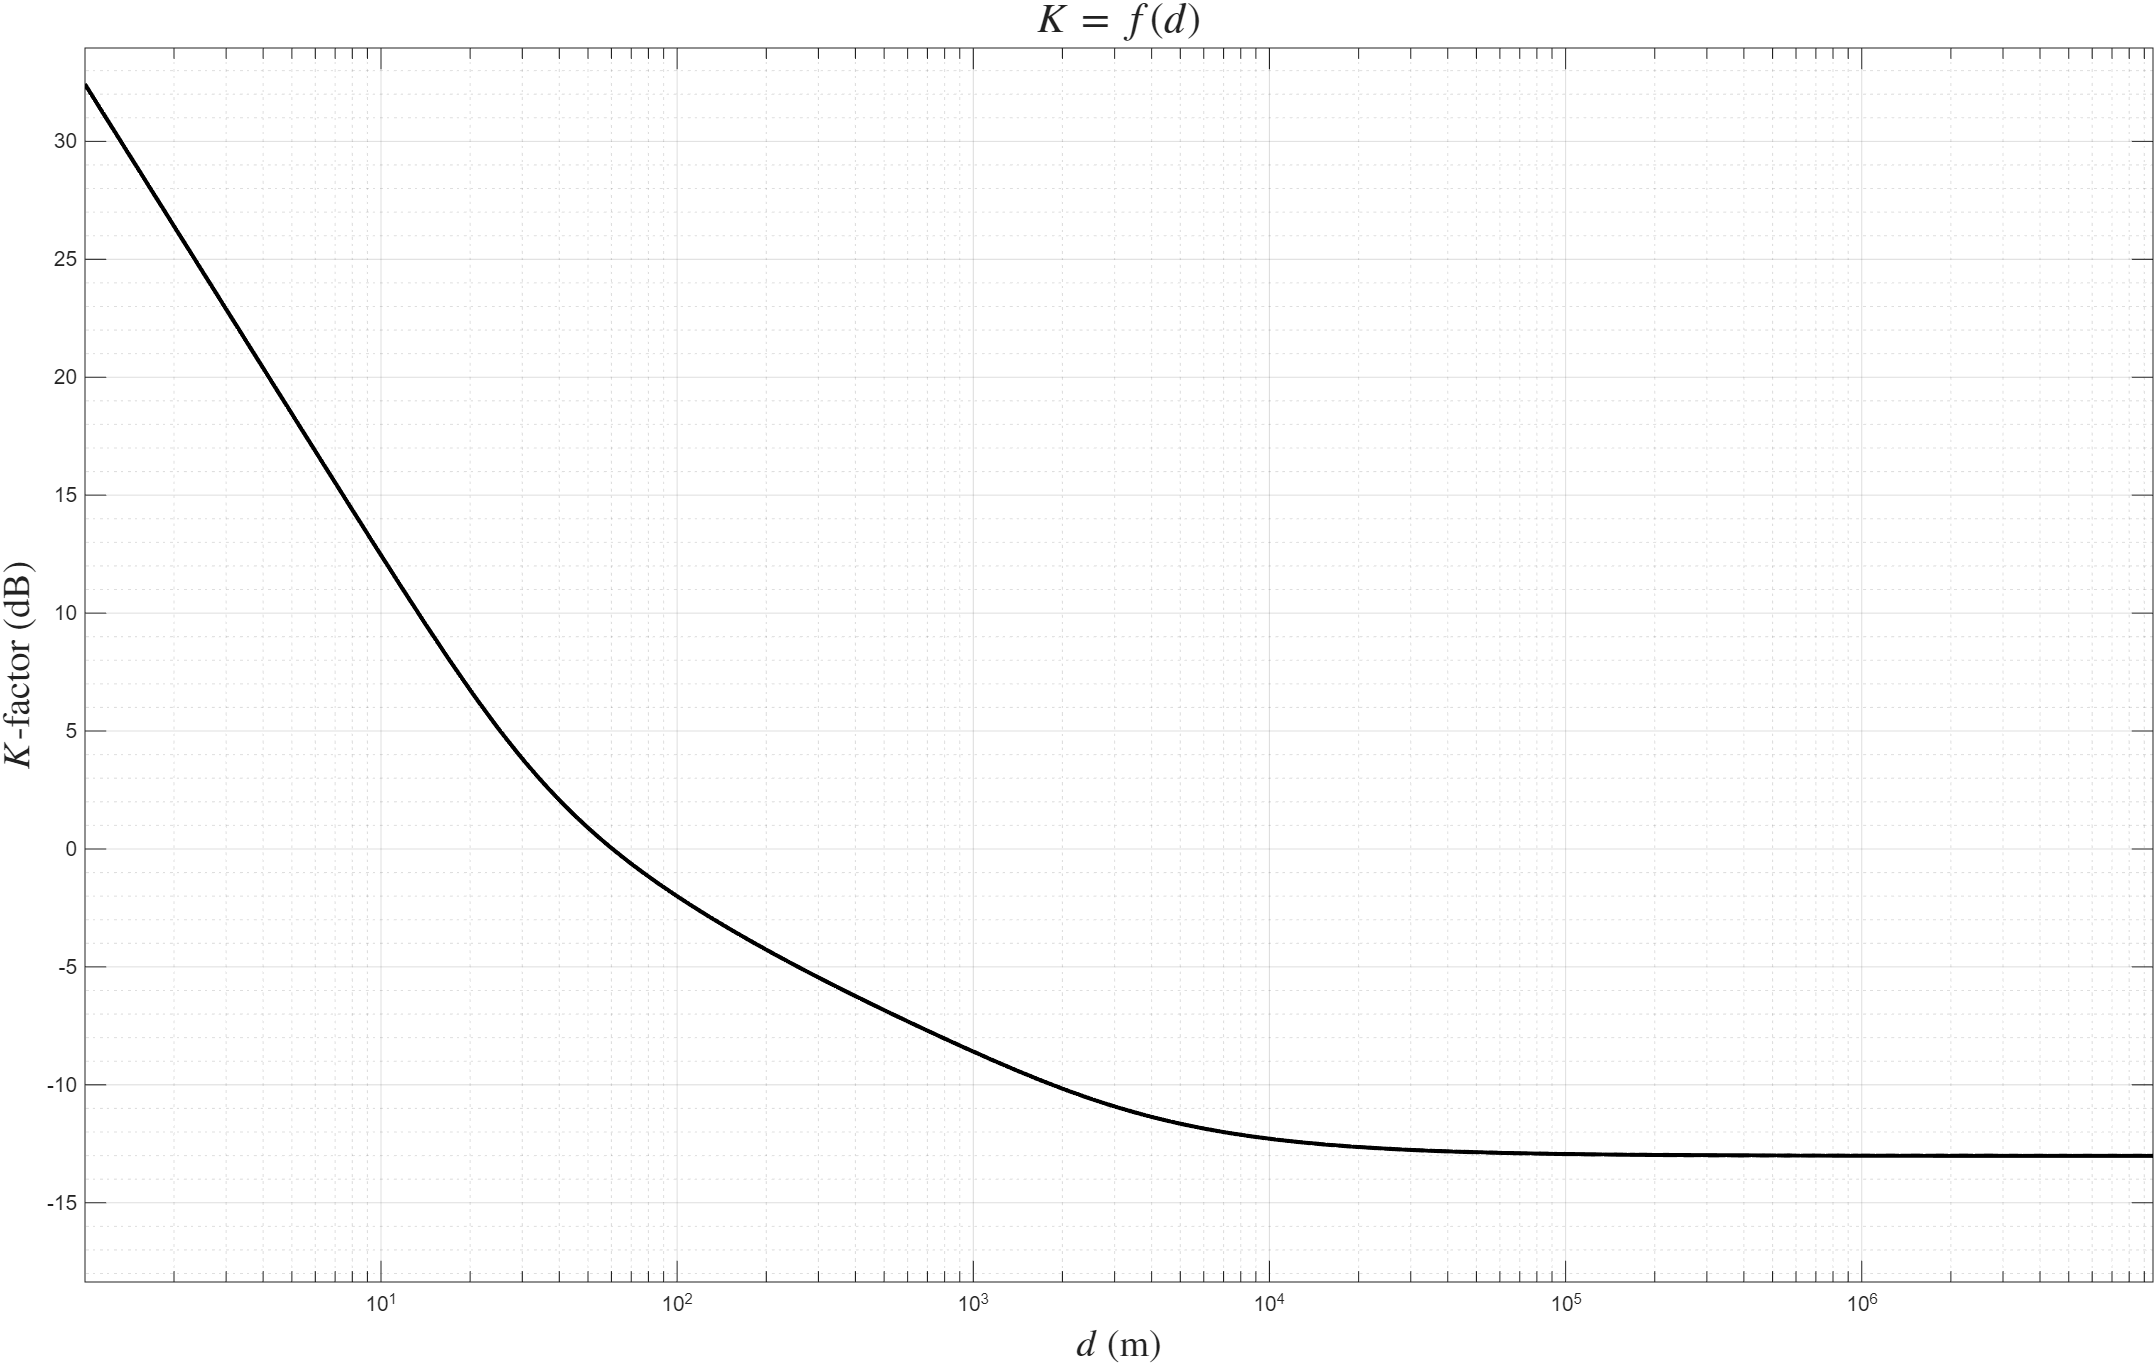
\includegraphics[width=\linewidth]{content/4-images/k-factor}
	\caption{K-factor as a function of the separation distance between TX and RX for $K=10$ reflections}
	\label{fig:k-factor}
\end{figure}

\section{Path Loss Model}
To analyze the large-scale path loss, small-scale fading caused by the rapid phase changes of the MPCs must be averaged out. This is done by computing the average received power, $\langle P_{RX} \rangle$, over local areas, defined as 5m segments. This averaging smooths out the fast fluctuations, revealing the slower trend of power decay with distance.
\begin{equation}
	\langle P_{RX}(d) \rangle = \frac{1}{5m} \int_{d-2.5m}^{d+2.5m} P_{RX}(x) dx
\end{equation}

The loss of the channel is defined as $L(d)$ such that:
\begin{align}
	\label{eq:loss}
	L(d) [dB] &= P_{TX} [dBm] - \langle P_{RX}(d) \rangle [dBm]\\
			  &= L_0(d) [dB] - 10 \log G_{TX} - 10 \log G_{RX}
\end{align}

Where $L_0(d)$ represent the part of the path loss that does not depend on the antenna. It can be from Equation \eqref{eq:loss} expressed as
\begin{equation}
	L_0(d) [dB] =  P_{TX} [dBm] + 10 \log G_{TX} + 10 \log G_{RX} - \langle P_{RX}(d) \rangle [dBm]
	\label{eq:loss-2}
\end{equation}

It is empirically proven that in general the path loss model follows a canonical form. The path loss model is fit into the canonical form and a linear regression is done:
\begin{align}
	L_0(d) [dB] &= L_0(d_0) + 10n \log\left(\frac{d}{d_0}\right)\\
				&= \underbrace{10n}_{slope} \log(d) + \underbrace{(L_0(d_0) - 10n \log(d_0))}_{intercept} \label{eq:lin-reg}
\end{align}


Where $d_0$ is a reference distance, and $n$ is the path loss exponent. This exponent describes how quickly the signal attenuates with distance on a large scale.

By combining Equation \eqref{eq:loss-2} and \eqref{eq:lin-reg}, $n$ and $L_0(d_0)$ can be found

\section{Variability $\sigma_L$}
The variability, or shadowing standard deviation $\sigma_L$, quantifies the variation of the actual received power around the path loss model prediction. It is calculated as the standard deviation of the difference (in dB) between the local-area averaged power and the path loss model prediction.
\begin{equation}
	\sigma_L^2 = \text{Var} \left[ 10\log(\langle P_{RX} \rangle) - (P_{TX}[dBm] - L(d)[dB]) \right]
\end{equation}

\section{Fade Margin and Cell Range}
Assuming the power variations around the path loss model are log-normally distributed, we can determine the fade margin ($M$) required to achieve a certain communication reliability. The reliability is the probability that the received power is above the receiver sensitivity ($P_{sens} = -70$ dBm).
\begin{equation}
	\text{Pr}(P_{RX} > P_{sens}) = \text{Reliability}
\end{equation}
The fade margin is the extra power (in dB) needed to overcome fading. The maximum allowable path loss for a given reliability is $L_{max} = P_{TX}[dBm] - P_{sens}[dBm] - M$. The cell range is the distance $d$ at which the path loss $L(d)$ equals this maximum allowable path loss. We can calculate the required margin for 50\%, 95\%, and 99\% reliability and the corresponding cell ranges.

\section{Interpretation of Results}
The introduction of reflections from buildings fundamentally changes the channel behavior compared to the simple LOS case.
\begin{itemize}
	\item \textbf{Multiray Fading:} The total received power is no longer a monotonic function of distance. The vector sum of the MPCs creates an interference pattern, causing rapid and deep fluctuations in signal strength (fading) as the distance $d$ changes. This is a critical feature of real-world urban channels.
	\item \textbf{Rician K-factor:} The K-factor provides a quantitative measure of the channel's nature. For short distances $d$, the LOS ray is much stronger than the reflected rays, resulting in a high K-factor and a Rician-like distribution with moderate fading. As $d$ increases, the LOS power decreases, and the reflected rays become relatively more significant, lowering the K-factor and making the channel behave more like a Rayleigh fading channel.
	\item \textbf{path loss Exponent:} The path loss exponent $n$ derived from the averaged power will likely be greater than 2 (the free-space value). This is because the multiray environment tends to confine the energy, creating a "waveguide" effect that can alter the rate of power decay with distance.
	\item \textbf{Fade Margin and Reliability:} The variability $\sigma_L$ necessitates a fade margin to ensure reliable communication. A higher desired reliability (e.g., 99\% vs. 95\%) requires a larger fade margin, which in turn reduces the maximum communication range for the system. This highlights the trade-off between reliability and coverage in a fading channel.
\end{itemize}

\chapter{LOS Channel - Wideband Analysis}
\label{chap:los_wide}

The analysis now transitions to the wideband case, where the signal's bandwidth is significant and can no longer be neglected. This requires moving from the narrowband model to models that explicitly account for the channel's behavior across the frequency band and in the time-delay domain.

\section{Impulse Response and Transfer Function}
For a single LOS ray, the physical channel is characterized by a single propagation path with delay $\tau_1$ and complex amplitude $\alpha_1$. The impulse response and transfer function are the same as those derived in the narrowband analysis, as they represent the underlying physical reality of the channel independent of signal bandwidth.

The physical impulse response is a single Dirac delta function, representing the instantaneous arrival of the signal after a delay $\tau_1$:
\begin{equation}
	h(\tau) = \alpha_1 \delta(\tau - \tau_1) = \left( j \frac{\lambda Z_0}{4\pi^2 R_a d_1} e^{-j2\pi f_c \tau_1} \right) \delta(\tau - \tau_1)
	\label{eq:los_impulse_response_wide}
\end{equation}
The corresponding transfer function, obtained via the Fourier transform of $h(\tau)$, is:
\begin{equation}
	H(f) = \alpha_1 e^{-j2\pi f \tau_1} = j \frac{\lambda Z_0}{4\pi^2 R_a d_1} e^{-j2\pi (f_c + f) \tau_1}
	\label{eq:los_transfer_function_wide}
\end{equation}
The magnitude of the impulse response is a single impulse, as shown in Figure \ref{fig:h_tau_los}. The magnitude of the transfer function, $|H(f)| = |\alpha_1|$, is constant across all frequencies, confirming that the LOS channel is frequency-flat, as depicted in Figure \ref{fig:Hf_los}.

\begin{figure}
	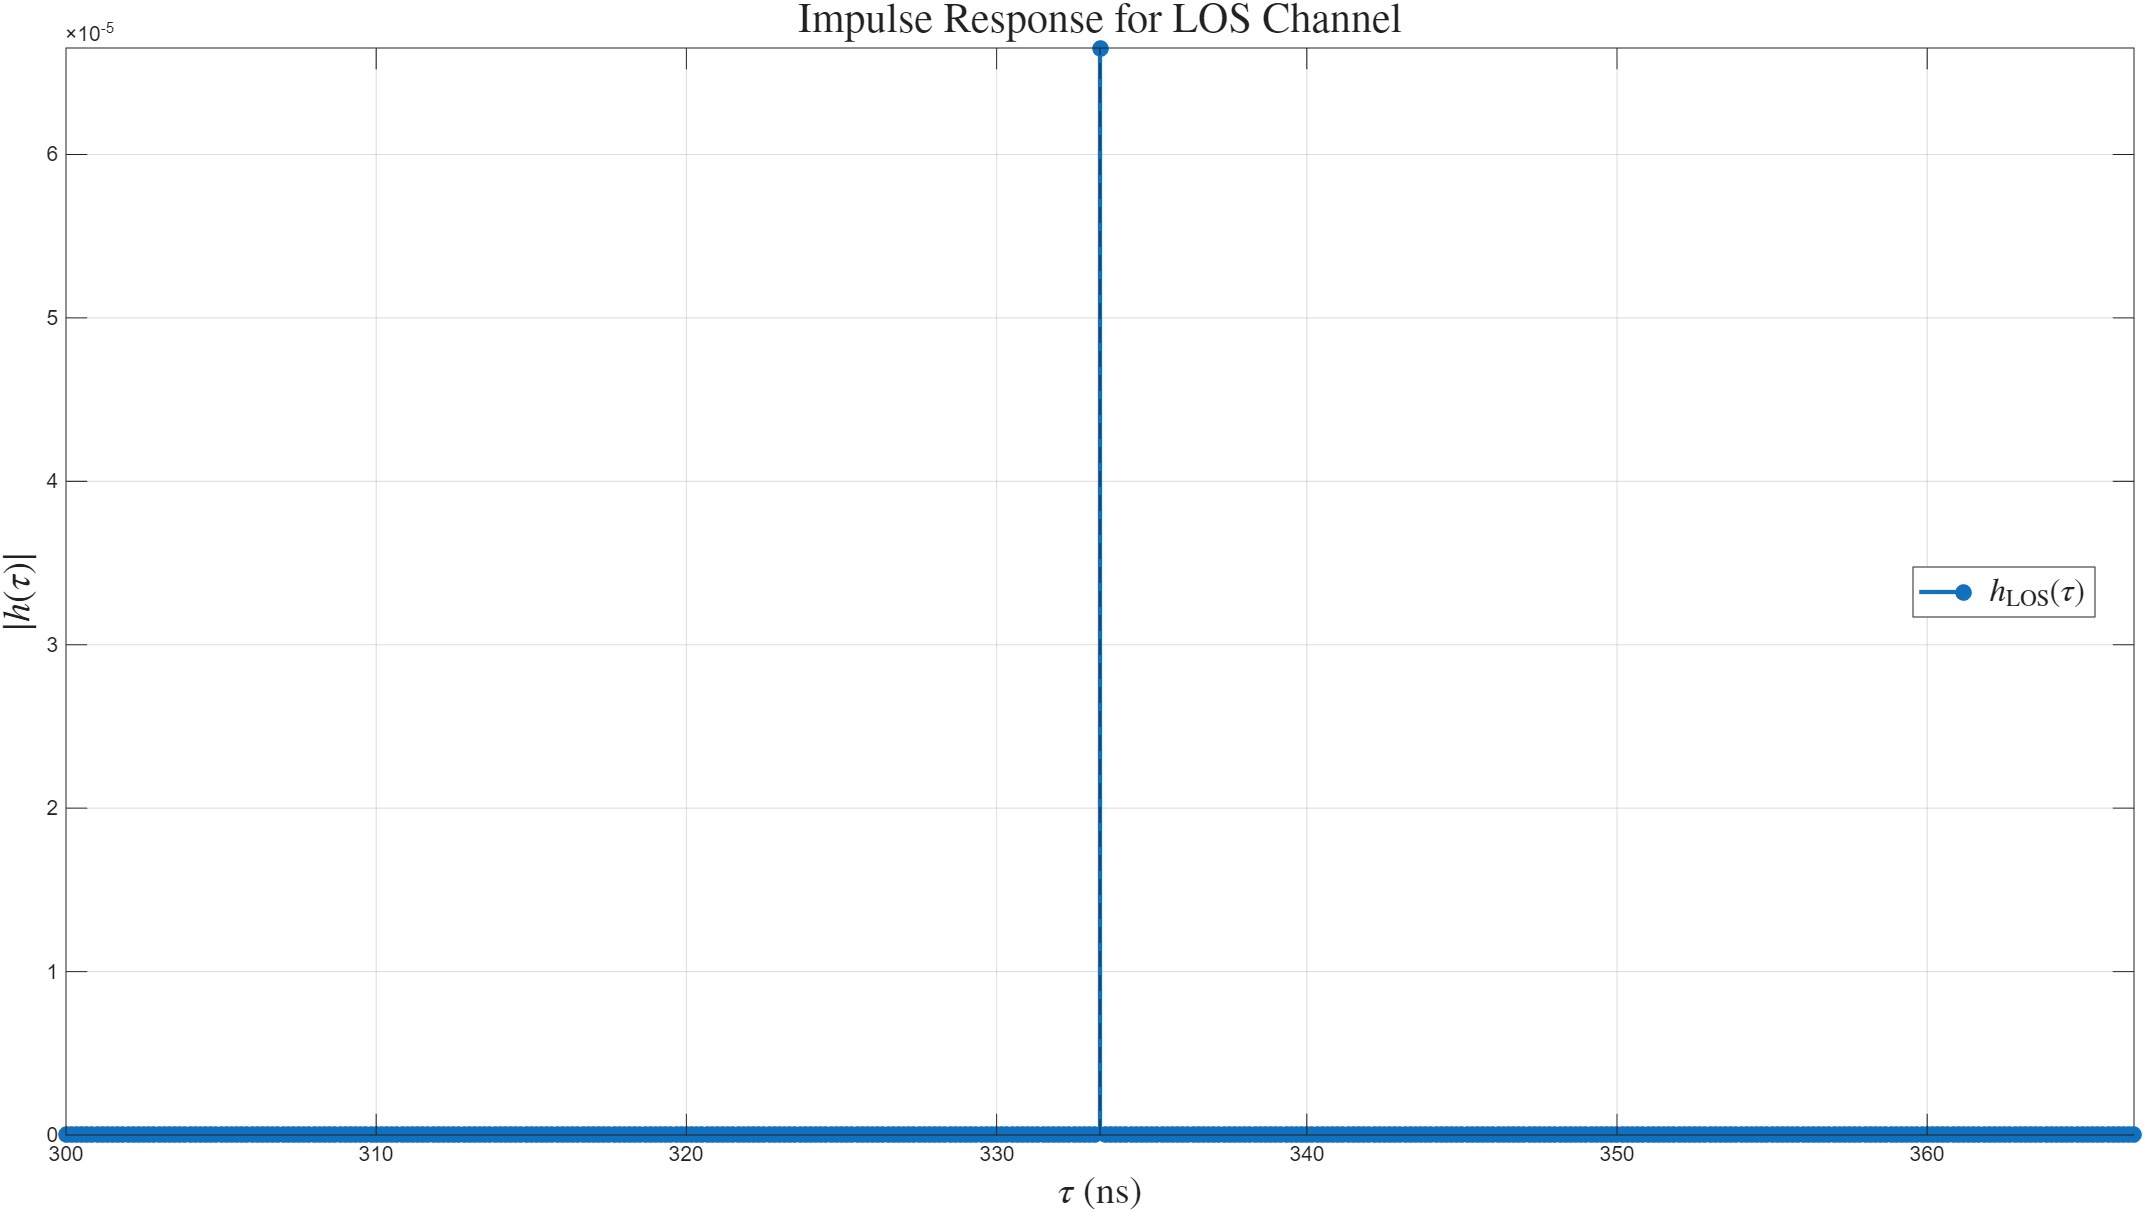
\includegraphics[width=\linewidth]{"content/4-images/h-tau-LOS.png"}
	\caption{Physical impulse response $|h(\tau)|$ for the LOS channel at $d=100$ m. The single impulse occurs at $\tau_1 = 333.33$ ns.}
	\label{fig:h_tau_los}
\end{figure}

\begin{figure}
	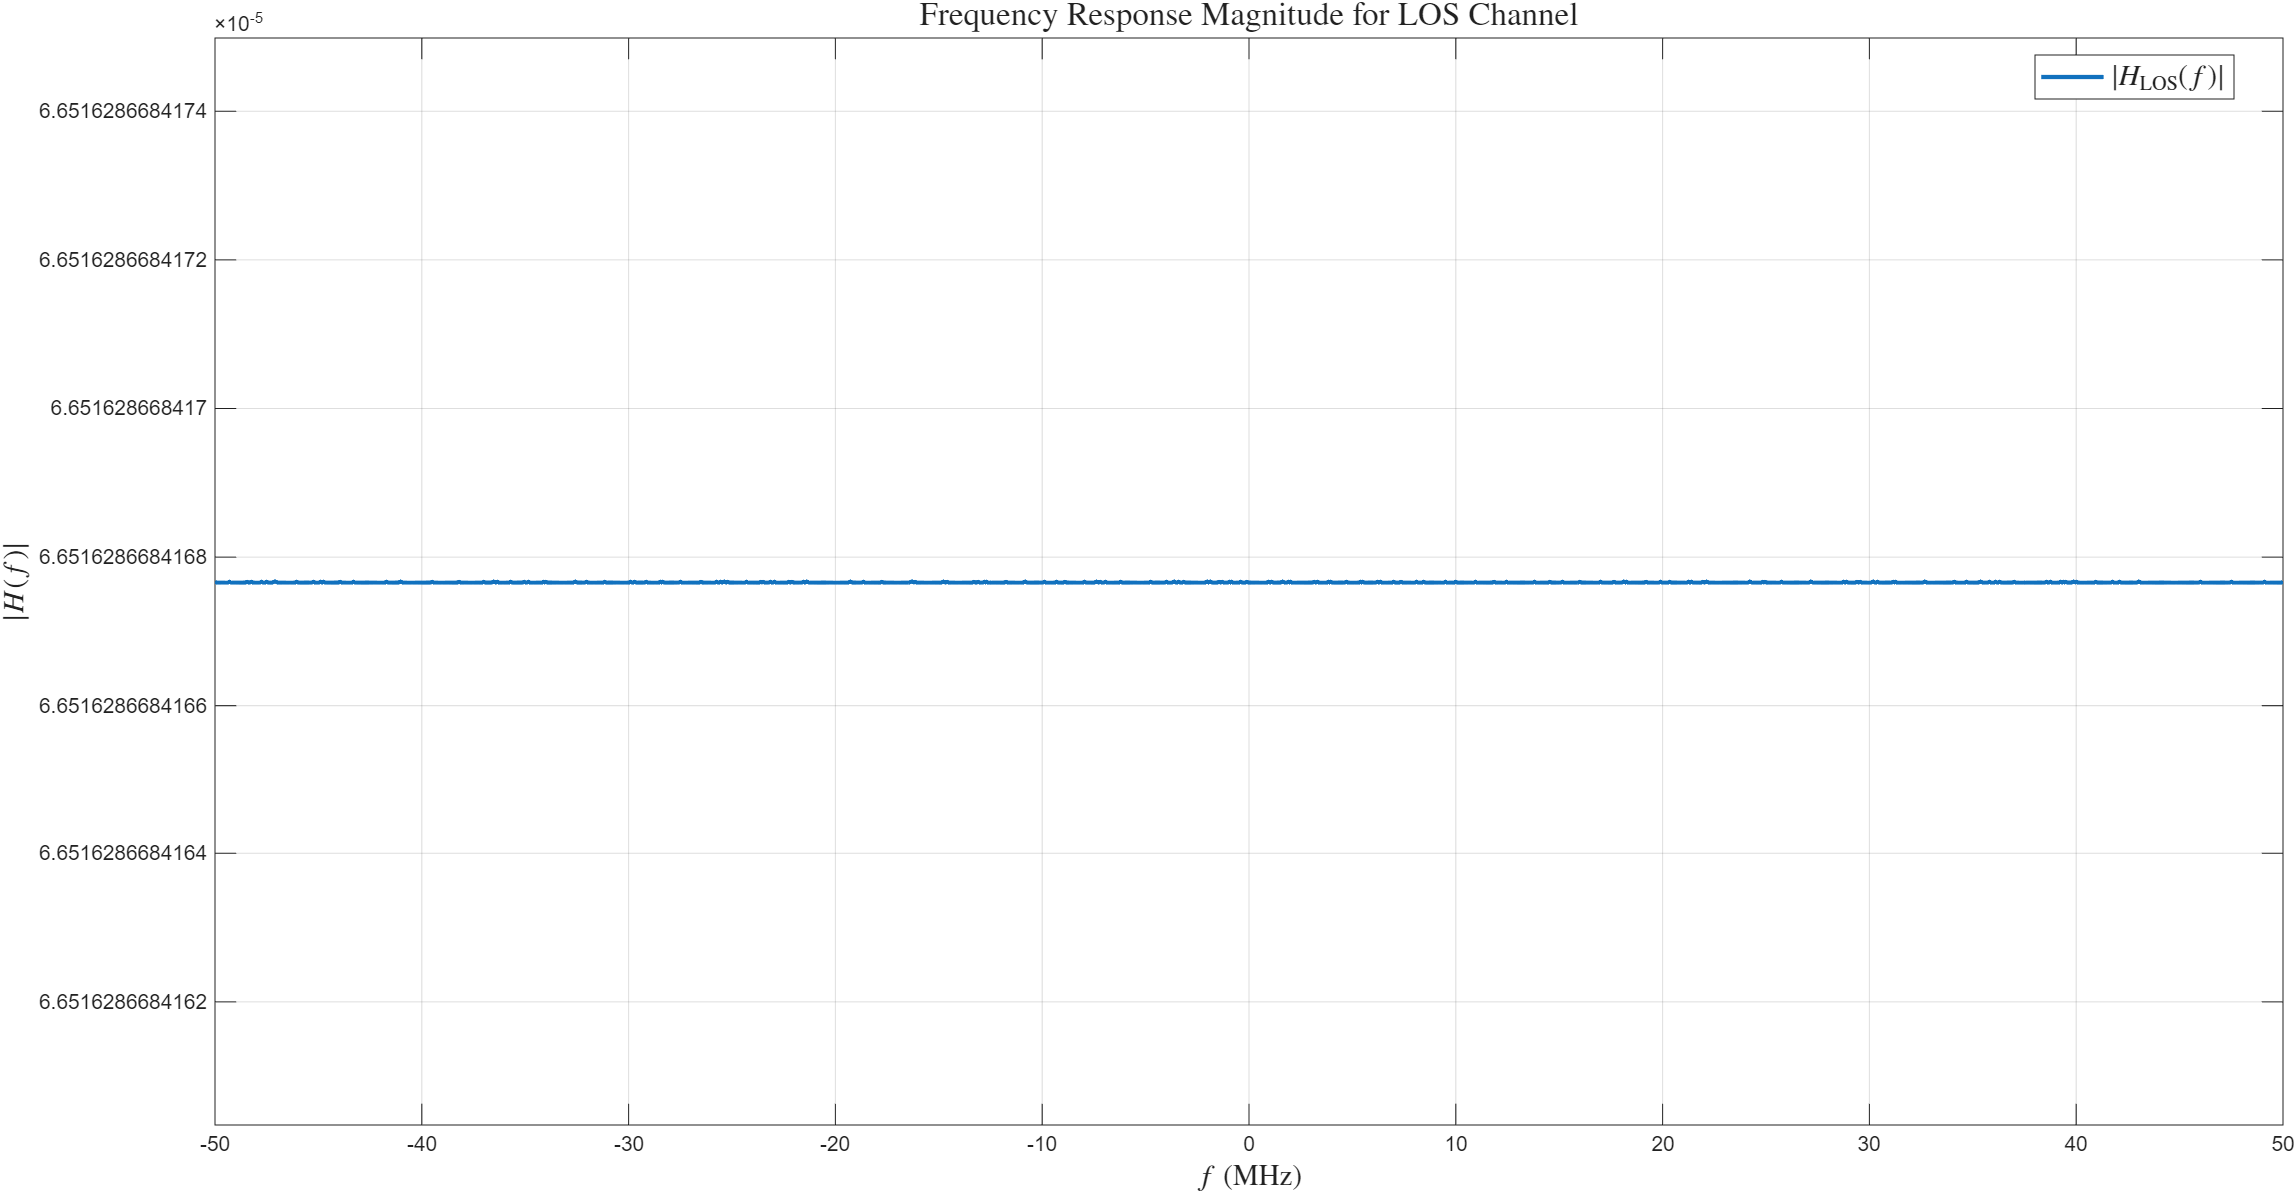
\includegraphics[width=\linewidth]{"content/4-images/Frequency Response H(f) - LOS.png"}
	\caption{Transfer function magnitude $|H(f)|$ for the LOS channel. The response is flat across the entire bandwidth.}
	\label{fig:Hf_los}
\end{figure}


\section{Tapped Delay Line Model $h_{TDL}(\tau)$}
The Tapped Delay Line model provides a discrete-time representation of the channel that accounts for the finite bandwidth $B$ of the communication system. The time resolution of the system is $\Delta\tau = 1/B$. The TDL impulse response is given by:
\begin{equation}
	h_{TDL}(\tau) = \sum_{l=0}^{L} h_l \delta(\tau - l\Delta\tau)
\end{equation}
where the complex gain of the $l$-th tap, $h_l$, is calculated by projecting the physical impulse response onto a basis of sinc functions:
\begin{equation}
	h_l = \int_0^{\infty} h(\tau) \operatorname{sinc}(B(\tau-l \Delta \tau)) d \tau
\end{equation}
Substituting the physical impulse response for the LOS channel, $h(\tau) = \alpha_1 \delta(\tau - \tau_1)$, into this integral gives:
\begin{equation}
	h_l = \int_0^{\infty} \alpha_1 \delta(\tau - \tau_1) \operatorname{sinc}(B(\tau-l \Delta \tau)) d \tau
\end{equation}
Using the sifting property of the Dirac delta function, the expression for the tap gains simplifies to:
\begin{equation}
	h_l = \alpha_1 \operatorname{sinc}(B(\tau_1 - l \Delta \tau))
\end{equation}
This equation shows that the gain of each tap is determined by the value of a sinc function centered at the physical delay $\tau_1$. For the simulation parameters ($B=100$ MHz, $\Delta\tau = 10$ ns), the LOS delay $\tau_1 = 333.33$ ns falls between the 33rd and 34th taps. The sinc function's main lobe will distribute the energy of the physical ray primarily across these adjacent taps, with smaller contributions to other taps, as shown in Figure \ref{fig:h_tdl_los}.

\begin{figure}[h!]
	\centering
	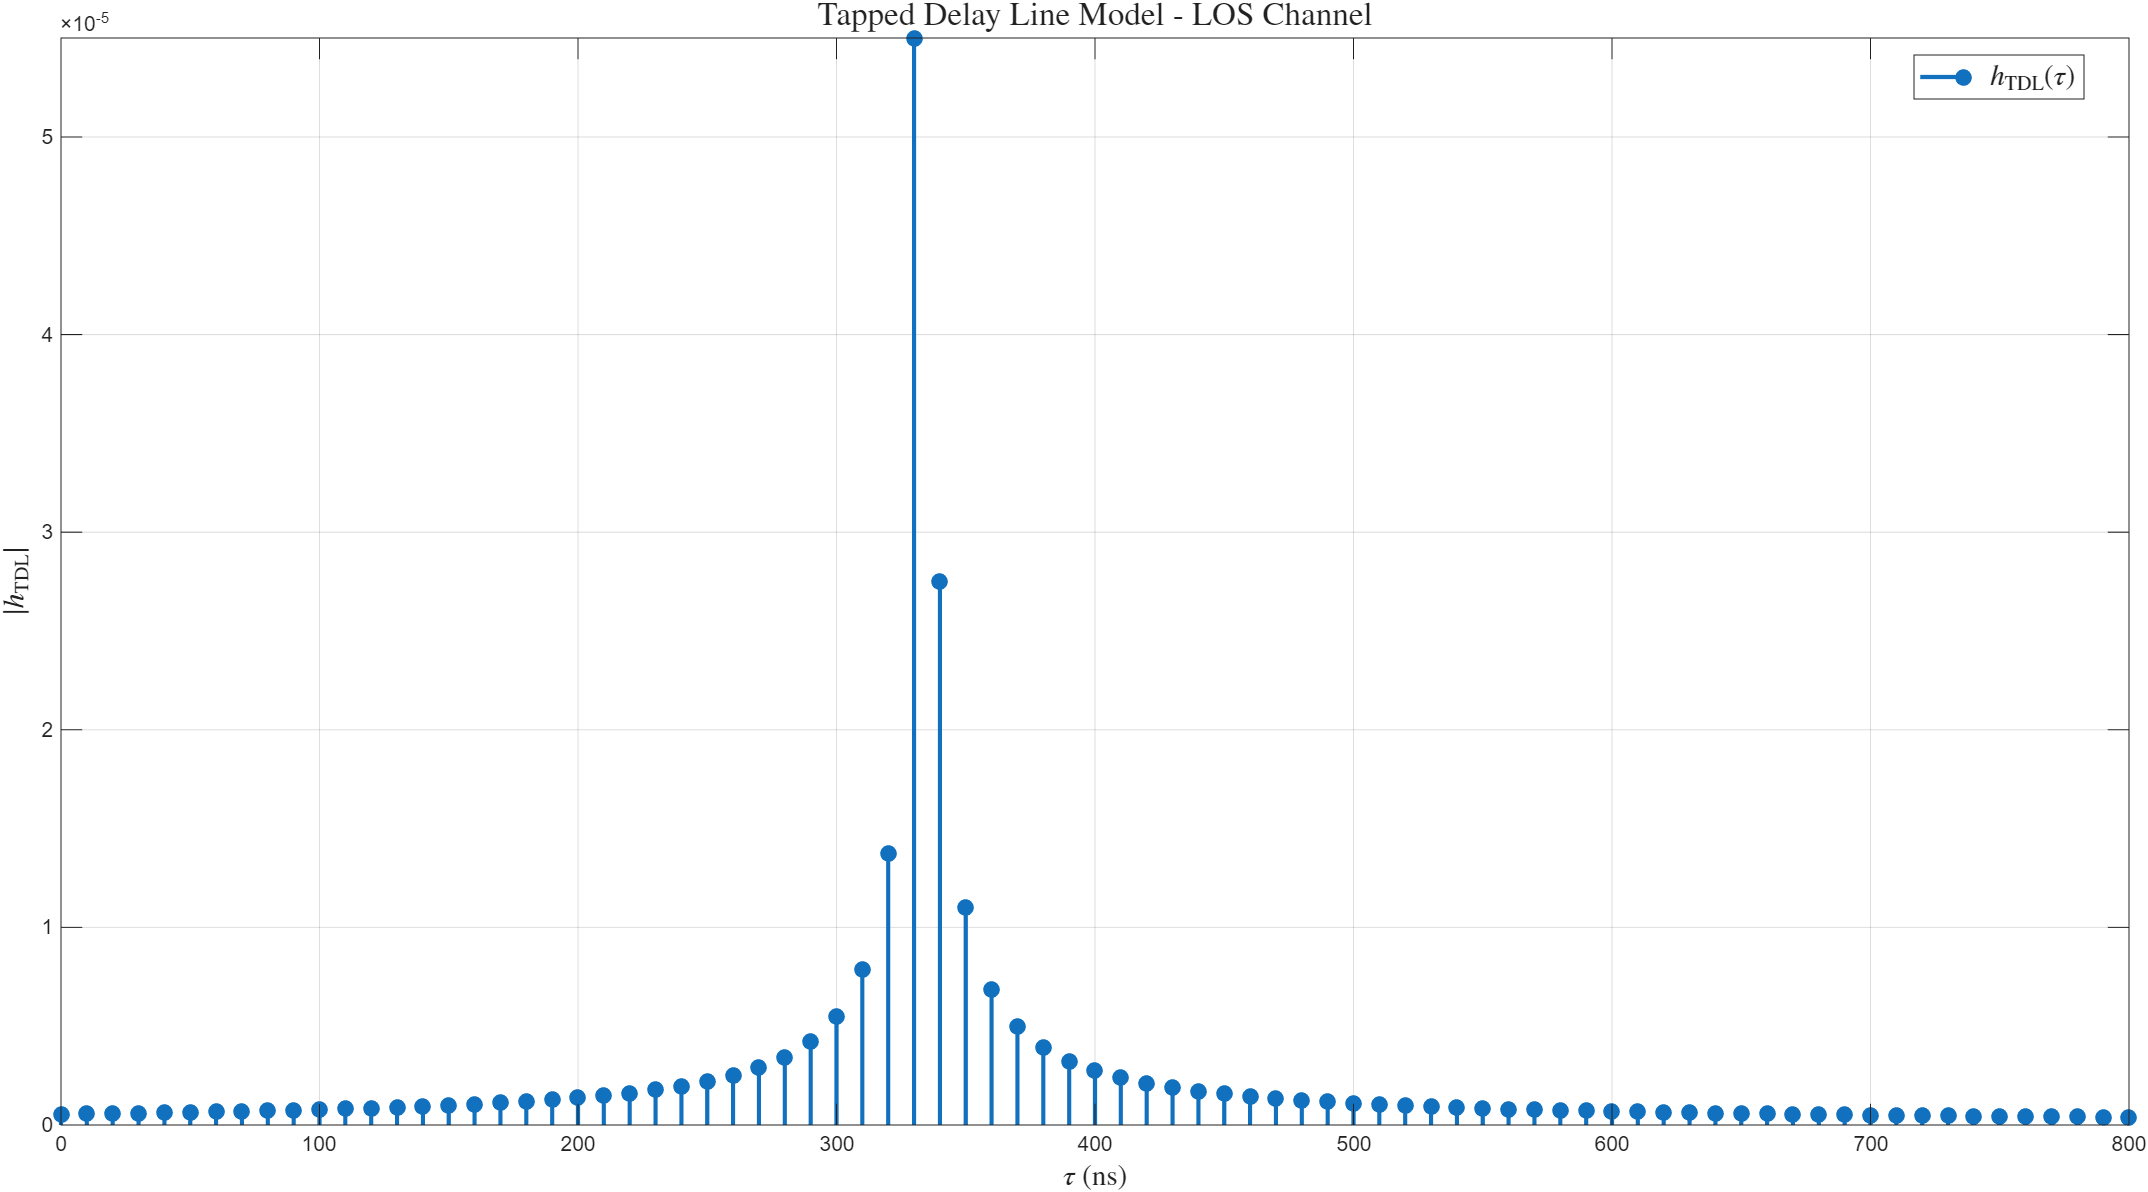
\includegraphics[width=\linewidth]{"content/4-images/Tapped Delay Line Model - LOS Channel.png"}
	\caption{Tapped Delay Line model $|h_{TDL}(\tau)|$ for the LOS channel. The energy of the single physical ray is spread across several discrete taps centered around the true delay $\tau_1$.}
	\label{fig:h_tdl_los}
\end{figure}

\section{Interpretation of Results}
The wideband analysis of the LOS channel provides several key insights:
\begin{itemize}
	\item \textbf{No Time Dispersion:} The physical impulse response consists of a single, sharp impulse. This signifies that there is no time dispersion in the channel; a transmitted impulse arrives as a single impulse at the receiver, albeit delayed and attenuated. This is the ideal channel condition.
	\item \textbf{Frequency-Flat Fading:} The lack of time dispersion directly results in a frequency-flat transfer function. Since $|H(f)|$ is constant, all frequency components of the transmitted signal are attenuated equally. The channel does not introduce any spectral distortion, which simplifies receiver design significantly.
	\item \textbf{TDL as a Band-Limited Model:} The TDL model illustrates the effect of the system's finite bandwidth. While the physical ray arrives at a precise moment $\tau_1$, the system with its limited time resolution $\Delta\tau$ perceives this energy as being spread across several discrete time intervals (taps). The sinc interpolation correctly models this effect, showing that the power is not confined to a single tap unless the physical delay happens to be an exact multiple of $\Delta\tau$.
\end{itemize}

\chapter{Full Channel, Wideband Analysis}
\label{chap:full_wide}

This section extends the wideband analysis to the full multiray channel, incorporating the  LOS ray and all significant reflected rays. The presence of multiple propagation paths with different delays introduces time dispersion, which fundamentally changes the channel's characteristics compared to the simple LOS case.

\section{Physical Impulse Response}
The physical impulse response of the full channel is the superposition of all $N$ MPCs. Each component is represented by a Dirac delta function located at its respective propagation delay $\tau_n$ and weighted by its complex amplitude $\alpha_n$.
\begin{equation}
	h(\tau) = \sum_{n=1}^{N} \alpha_n \delta(\tau - \tau_n)
\end{equation}
where $\alpha_n$ accounts for path loss, phase rotation due to propagation, and the cumulative effect of reflection coefficients. Unlike the LOS case, which has a single impulse, the full channel response is a train of impulses spread over time, as shown in Figure \ref{fig:h_tau_full}. This spread is known as the channel's \textbf{time dispersion}. The simulation for $d=100$ m and up to $M=10$ reflections identifies $N=21$ distinct MPCs.

\begin{figure}[h!]
	\centering
	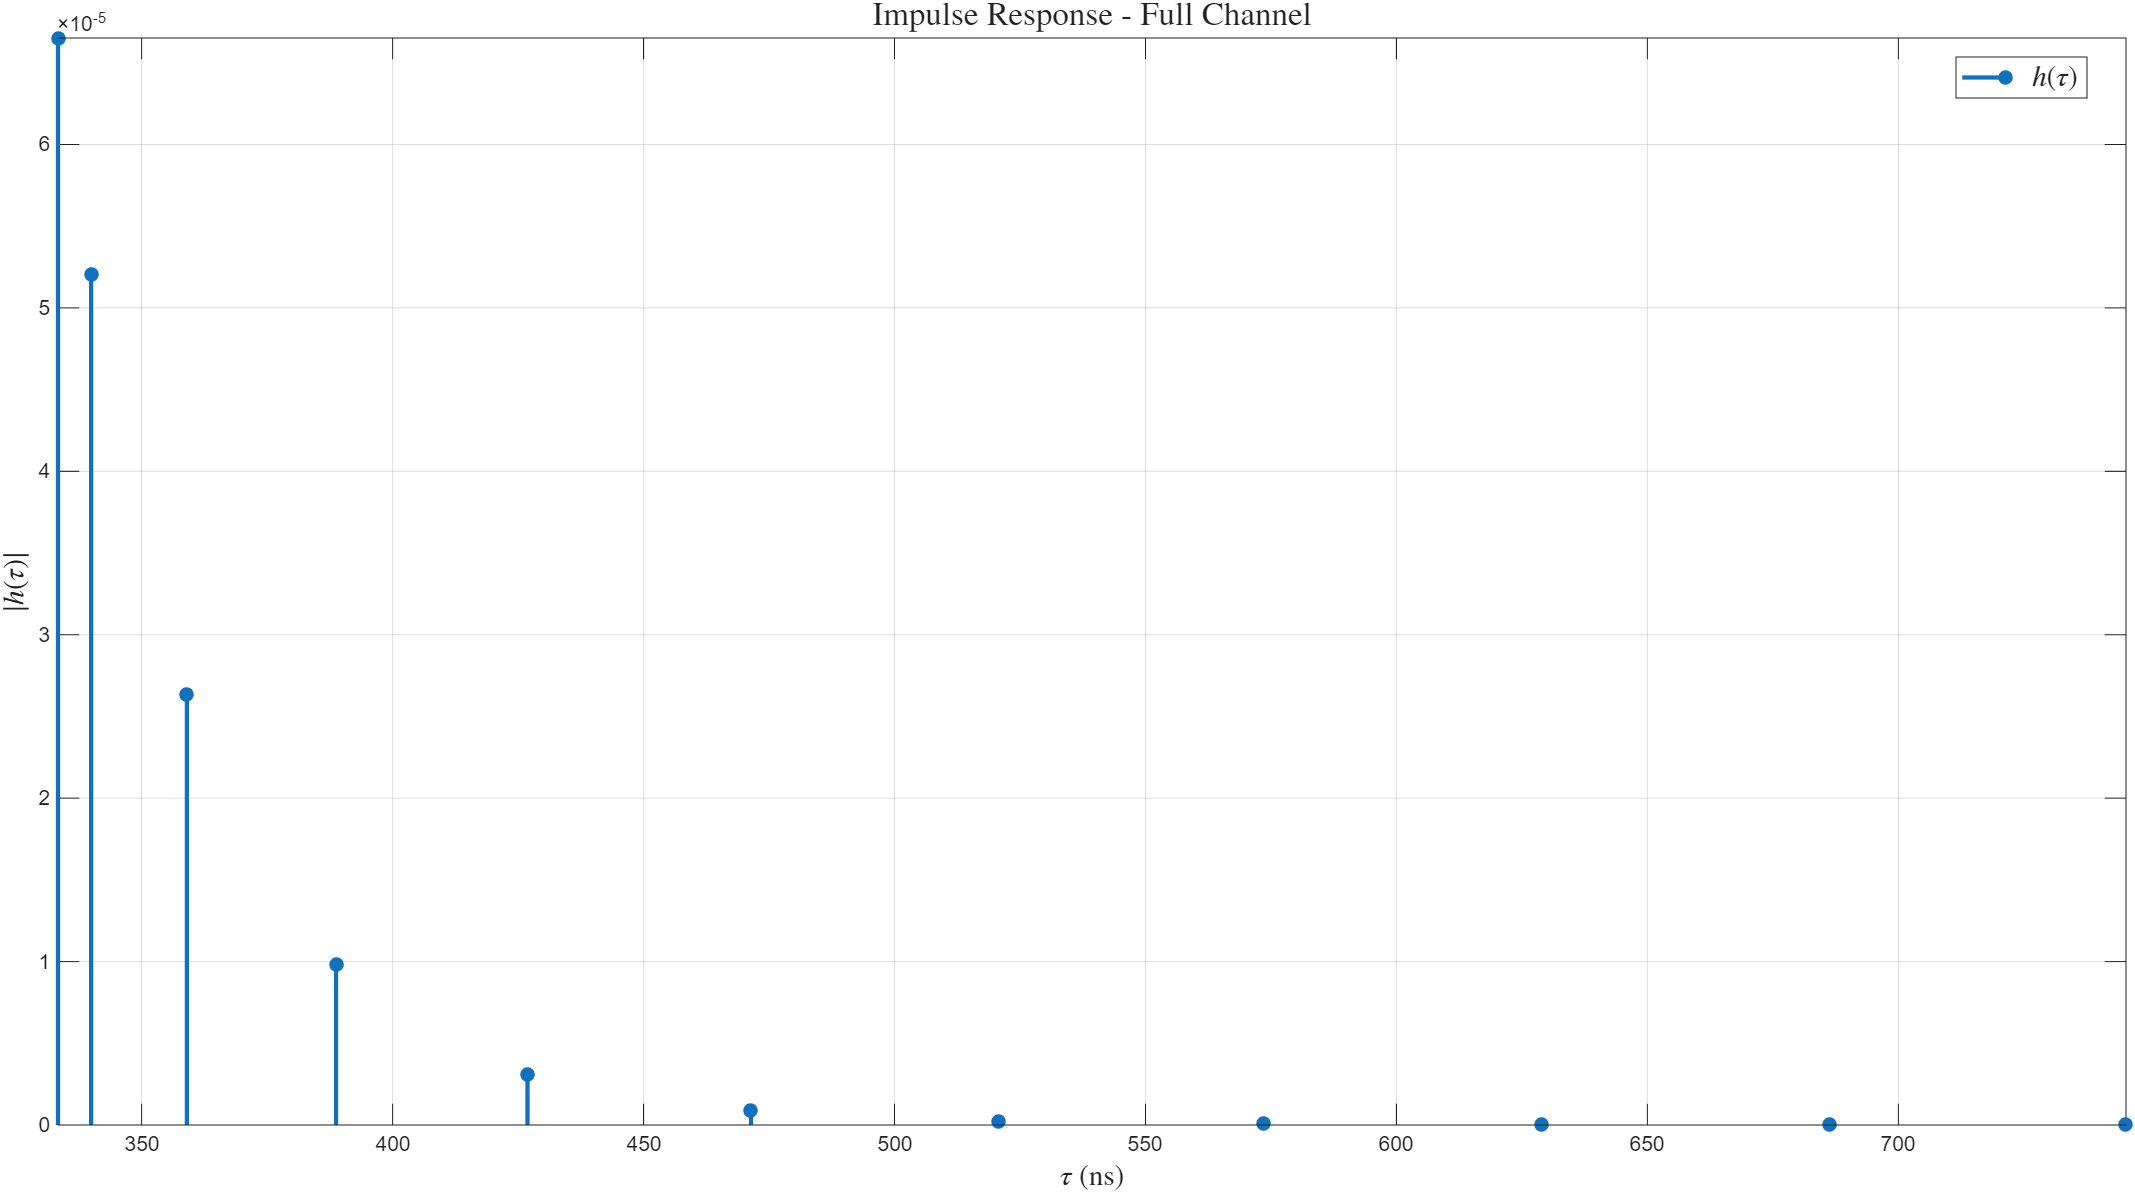
\includegraphics[width=\linewidth]{"content/4-images/h-tau - Full Channel.png"}
	\caption{Physical impulse response $|h(\tau)|$ for the full channel at $d=100$ m. The multiple impulses represent the various MPCs arriving at different delays, illustrating time dispersion.}
	\label{fig:h_tau_full}
\end{figure}

\section{Transfer Function $H(f)$}
The transfer function $H(f)$ is the Fourier transform of the physical impulse response $h(\tau)$:
\begin{align}
	H(f) &= \mathcal{FT}\left\{ \sum_{n=1}^{N} \alpha_n \delta(\tau - \tau_n) \right\} \\
	&= \sum_{n=1}^{N} \alpha_n \mathcal{FT}\left\{ \delta(\tau - \tau_n) \right\} \\
	&= \sum_{n=1}^{N} \alpha_n e^{-j2\pi f \tau_n}
	\label{eq:full_transfer_function_wide}
\end{align}
The transfer function is now a sum of complex phasors. As the frequency $f$ varies, the relative phases of these components change, leading to constructive and destructive interference. This causes the magnitude of the transfer function, $|H(f)|$, to vary significantly across the bandwidth, a phenomenon known as \textbf{frequency-selective fading}. As seen in Figure \ref{fig:Hf_full}, the channel exhibits deep nulls at frequencies where the MPCs combine destructively.

\begin{figure}[h!]
	\centering
	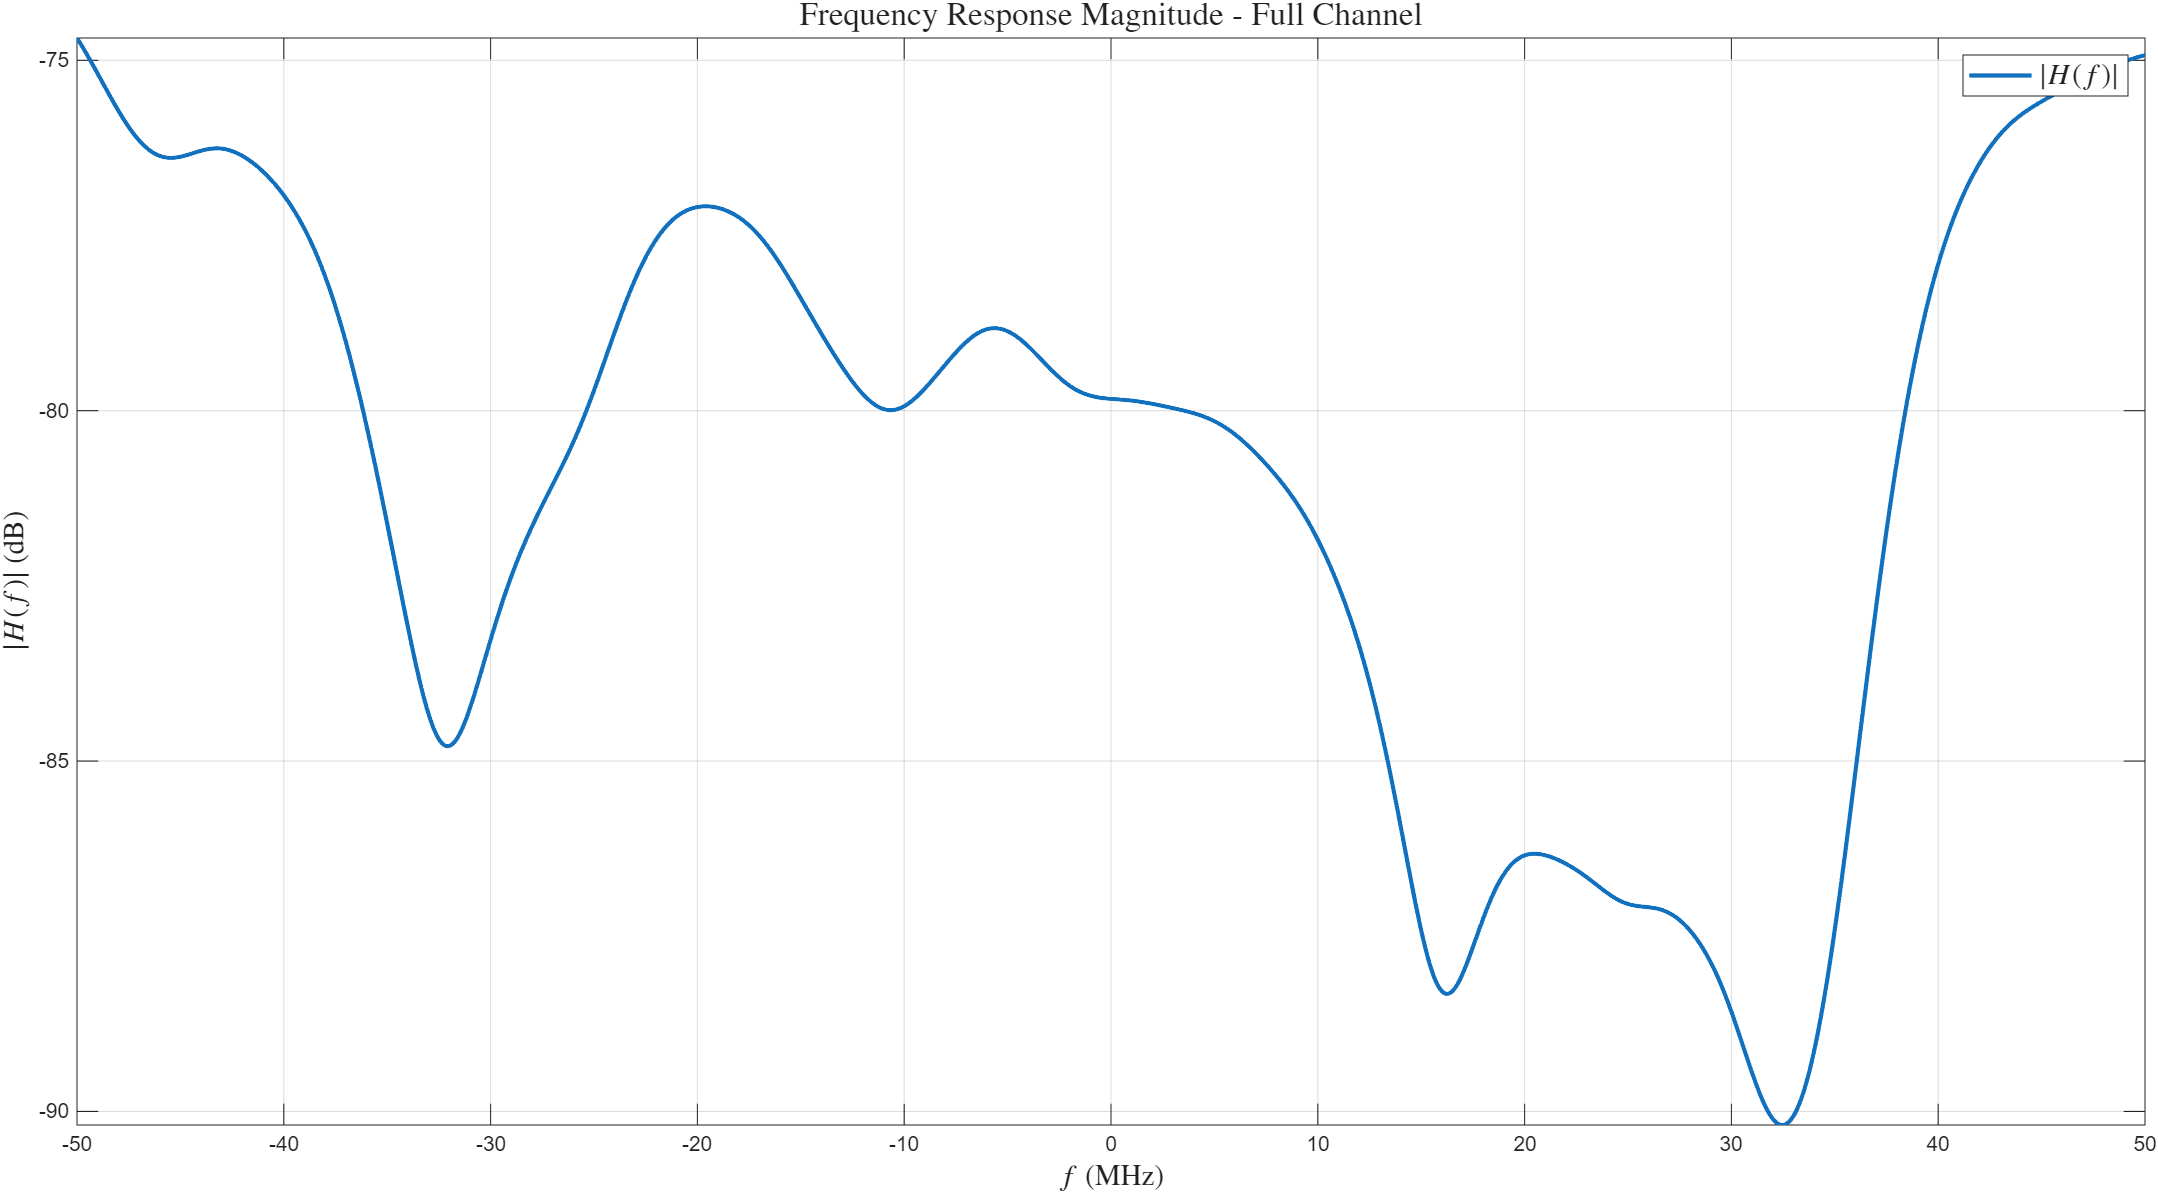
\includegraphics[width=\linewidth]{"content/4-images/Frequency Response H(f) - Full Channel.png"}
	\caption{Transfer function magnitude $|H(f)|$ for the full channel. The constructive and destructive interference of the MPCs creates deep nulls, illustrating frequency-selective fading.}
	\label{fig:Hf_full}
\end{figure}

\section{Tapped Delay Line Model $h_{TDL}(\tau)$}
As in the LOS case, the TDL model provides a practical, band-limited representation of the channel. The gain of the $l$-th tap, $h_l$, is found by integrating the full physical impulse response against the sinc function:
\begin{align}
	h_l &= \int_0^{\infty} h(\tau) \operatorname{sinc}(B(\tau-l \Delta \tau)) d \tau \\
	&= \int_0^{\infty} \left( \sum_{n=1}^{N} \alpha_n \delta(\tau - \tau_n) \right) \operatorname{sinc}(B(\tau-l \Delta \tau)) d \tau
\end{align}
Applying the sifting property of the delta function for each term in the sum yields:
\begin{equation}
	\boxed{h_l = \sum_{n=1}^{N} \alpha_n \operatorname{sinc}(B(\tau_n - l \Delta \tau))}
\end{equation}
Each tap gain $h_l$ is now a coherent sum of all physical MPCs, weighted by how close their delays $\tau_n$ are to the tap position $l\Delta\tau$. This model effectively groups the physical rays into discrete time bins, with the complex gain of each bin representing the vector sum of the rays falling within it. The resulting TDL impulse response, shown in Figure \ref{fig:h_tdl_full}, has significant energy spread across multiple taps, directly reflecting the time-dispersive nature of the physical channel.

\begin{figure}[h!]
	\centering
	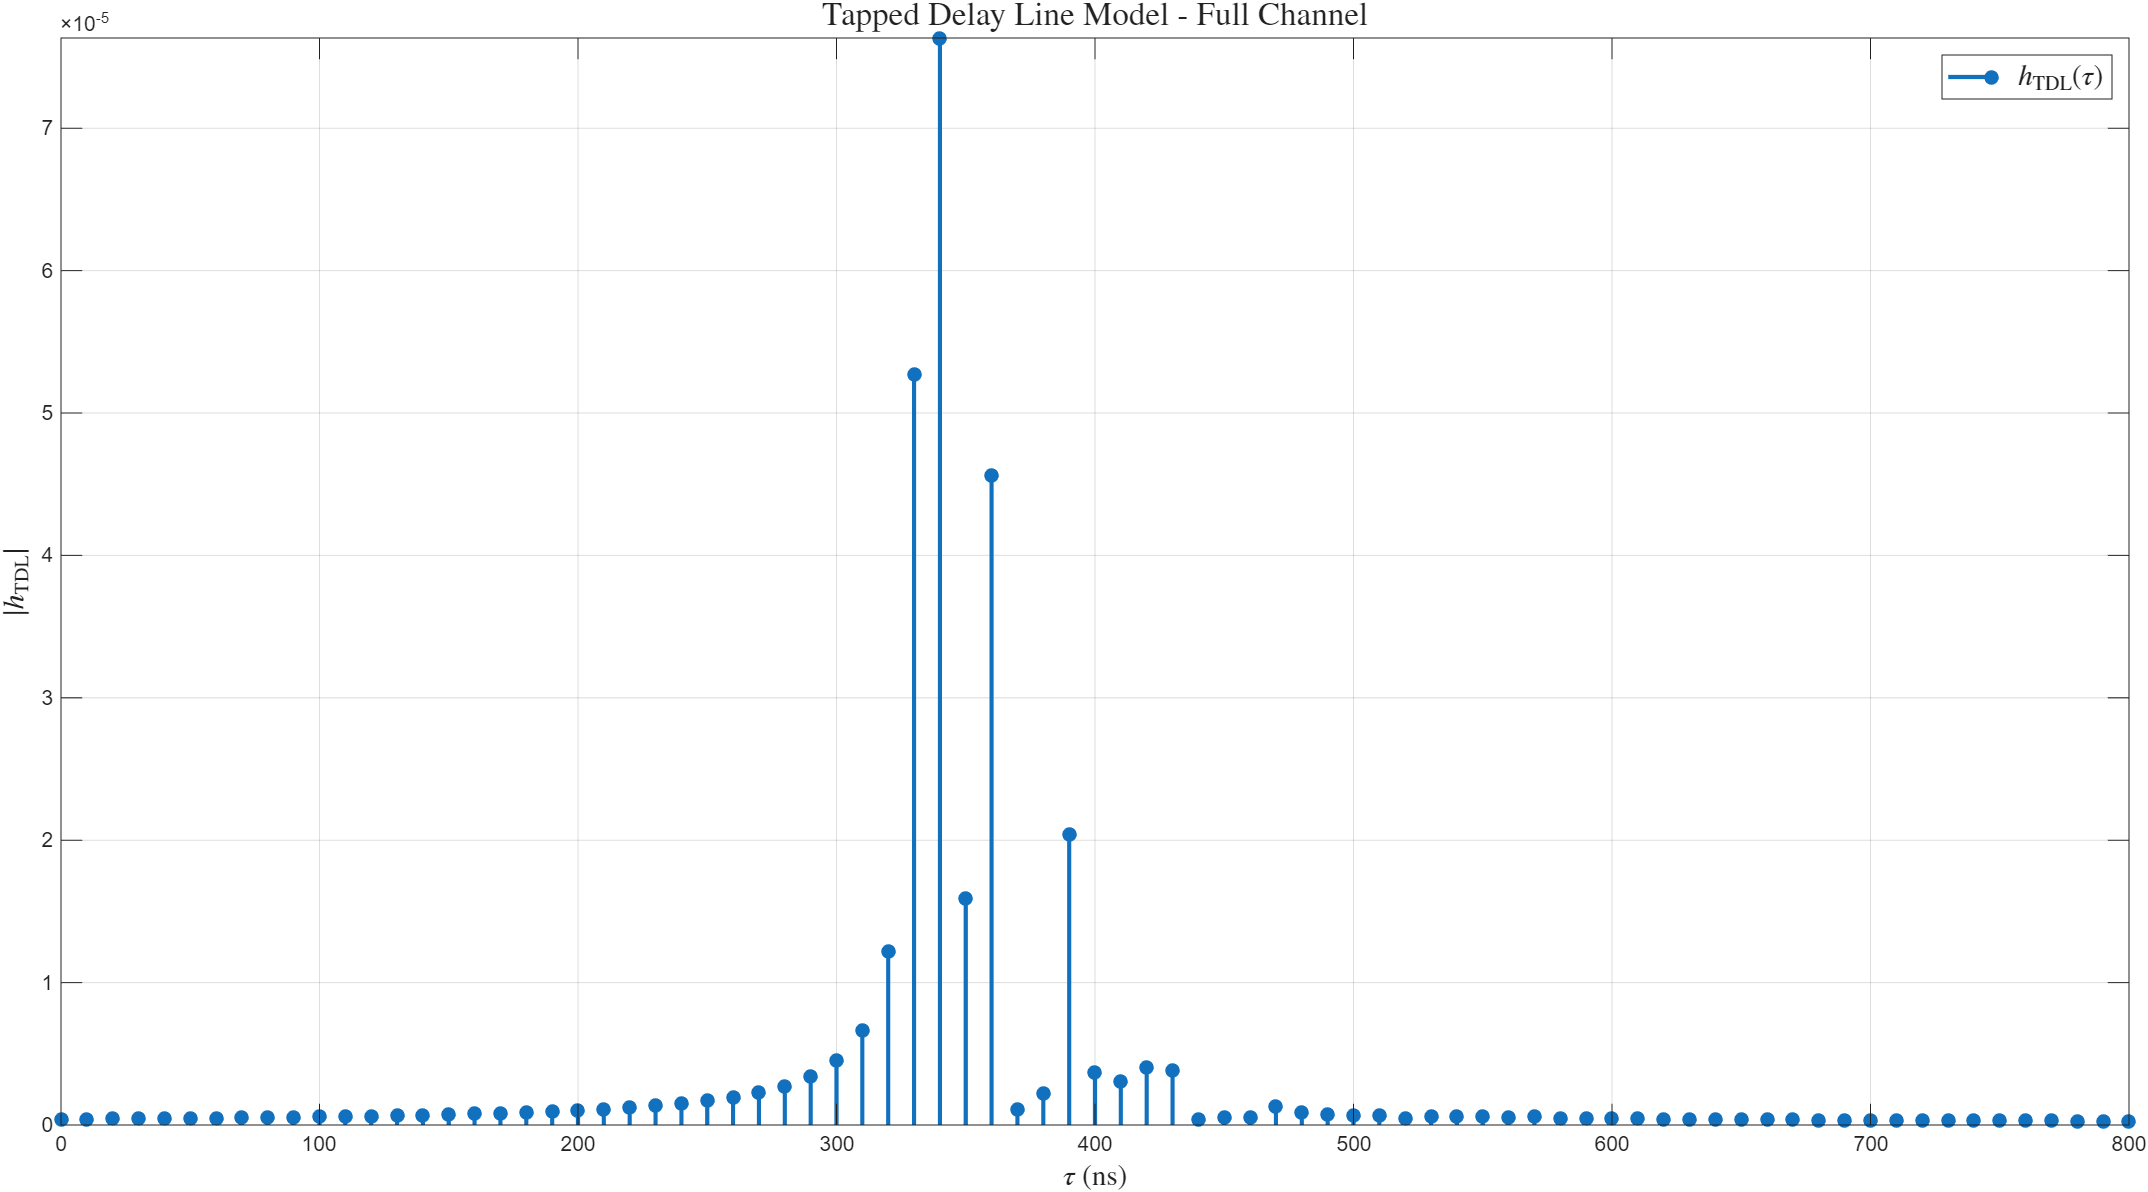
\includegraphics[width=\linewidth]{"content/4-images/Tapped Delay Line Model - Full Channel.png"}
	\caption{Tapped Delay Line model $|h_{TDL}(\tau)|$ for the full channel. The energy from the 21 MPCs is distributed across numerous taps, creating a discrete-time profile that mirrors the physical channel's delay spread.}
	\label{fig:h_tdl_full}
\end{figure}

\section{Interpretation of Results}
The wideband analysis of the full multiray channel reveals the fundamental challenges of wireless communication in such environments:
\begin{itemize}
	\item \textbf{Time Dispersion and Intersymbol Interference (ISI):} The physical impulse response in Figure \ref{fig:h_tau_full} shows that a transmitted impulse is received as a series of echoes spread out in time. This delay spread means that the energy from one transmitted symbol will spill over into the time slots of subsequent symbols, causing Intersymbol Interference (ISI). ISI is a major source of errors in digital communications and requires complex equalization techniques at the receiver to mitigate.
	\item \textbf{Frequency-Selective Fading:} The time dispersion is the direct cause of the frequency-selective fading observed in Figure \ref{fig:Hf_full}. The deep nulls in the channel's frequency response can completely wipe out parts of the signal's spectrum. If important information is located at these frequencies, it can be lost. This is why wideband systems often employ techniques like Orthogonal Frequency Division Multiplexing (OFDM), which divides the data into many narrow sub-carriers, making the system more robust to these selective fades.
	\item \textbf{TDL as a Practical Channel Model:} The TDL model (Figure \ref{fig:h_tdl_full}) is a powerful and practical tool. It captures the essential time-dispersive nature of the channel in a discrete format that is directly usable in system-level simulations and for designing digital equalizers. The number of significant taps in the TDL model is a direct measure of the severity of the channel's memory and the complexity required for the equalizer.
\end{itemize}

\input{content/1-project/6-further}
\input{content/1-project/7-conclu}


%Bibliography
\nocite{*}
\printbibliography[type=article,title=Articles]

\end{document}
